\documentclass[unicode,11pt,a4paper,oneside,numbers=endperiod,openany]{scrartcl}
\usepackage{minted}
\usepackage[fleqn]{amsmath}
\usepackage{amssymb}
\usepackage{xcolor}
\usepackage{caption}


\usepackage{ifthen}
\usepackage[utf8]{inputenc}
\usepackage{graphics}
\usepackage{graphicx}
\usepackage{hyperref}
\usepackage{amsmath}

\pagestyle{plain}
\voffset -5mm
\oddsidemargin  0mm
\evensidemargin -11mm
\marginparwidth 2cm
\marginparsep 0pt
\topmargin 0mm
\headheight 0pt
\headsep 0pt
\topskip 0pt        
\textheight 255mm
\textwidth 165mm

\newcommand{\duedate} {}
\newcommand{\setduedate}[1]{%
\renewcommand\duedate {Due date:~ #1}}
\newcommand\isassignment {false}
\newcommand{\setassignment}{\renewcommand\isassignment {true}}
\newcommand{\ifassignment}[1]{\ifthenelse{\boolean{\isassignment}}{#1}{}}
\newcommand{\ifnotassignment}[1]{\ifthenelse{\boolean{\isassignment}}{}{#1}}

\newcommand{\assignmentpolicy}{
\begin{table}[h]
\begin{center}
\scalebox{0.8} {%
\begin{tabular}{|p{0.02cm}p{16cm}|}
\hline
&\\
\multicolumn{2}{|c|}{\Large\textbf{Numerical Computing 2022 ---  Submission Instructions}}\\
\multicolumn{2}{|c|}{\large\textbf{(Please, notice that following instructions are mandatory: }}\\
\multicolumn{2}{|c|}{\large\textbf{submissions that don't comply with, won't be considered)}}\\
&\\
\textbullet & Assignments must be submitted to \href{https://www.icorsi.ch/course/view.php?id=14666}{iCorsi} (i.e. in electronic format).\\
\textbullet & Provide both executable package and sources (e.g. C/C++ files, Julia). 
If you are using libraries, please add them in the file. Sources must be organized in directories called:\\
\multicolumn{2}{|c|}{\textit{Project\_number\_lastname\_firstname}}\\
& and  the  file must be called:\\
\multicolumn{2}{|c|}{\textit{project\_number\_lastname\_firstname.zip}}\\
\multicolumn{2}{|c|}{\textit{project\_number\_lastname\_firstname.pdf}}\\
\textbullet &  The TAs will grade your project by reviewing your project write-up, and looking at the implementation you attempted, and benchmarking your code's performance.\\

\textbullet & You are allowed to discuss all questions with anyone you like; however: (i) your submission must list anyone you discussed problems with and (ii) you must write up your submission independently.\\
\hline
\end{tabular}
}
\end{center}
\end{table}
}
\newcommand{\punkte}[1]{\hspace{1ex}\emph{\mdseries\hfill(#1~\ifcase#1{Points}\or{Points}\else{Points}\fi)}}


\newcommand\serieheader[6]{
\thispagestyle{empty}%
\begin{flushleft}

\includegraphics[width=0.45\textwidth]{CI_logo}
\end{flushleft}
  \noindent%
  {\large\ignorespaces{\textbf{#1}}\hspace{\fill}\ignorespaces{ \textbf{#2}}}\\ \\%
  {\large\ignorespaces #3 \hspace{\fill}\ignorespaces #4}\\
  \noindent%
  \bigskip
  \hrule\par\bigskip\noindent%
  \bigskip {\ignorespaces {\Large{\textbf{#5}}}
  \hspace{\fill}\ignorespaces \large \ifthenelse{\boolean{\isassignment}}{\duedate}{#6}}
  \hrule\par\bigskip\noindent%  \linebreak
 }

\makeatletter
\def\enumerateMod{\ifnum \@enumdepth >3 \@toodeep\else
      \advance\@enumdepth \@ne
      \edef\@enumctr{enum\romannumeral\the\@enumdepth}\list
      {\csname label\@enumctr\endcsname}{\usecounter
        {\@enumctr}%%%? the following differs from "enumerate"
	\topsep0pt%
	\partopsep0pt%
	\itemsep0pt%
	\def\makelabel##1{\hss\llap{##1}}}\fi}
\let\endenumerateMod =\endlist
\makeatother




\usepackage{textcomp}


\newcommand{\bmat}[1]{
   \ensuremath{
   \begin{bmatrix}
       #1
   \end{bmatrix}
}}


\begin{document}


\setassignment
\setduedate{Wednesday, November 9, 2022, 11:59 PM}

\serieheader{Numerical Computing}{2022}{Student: Albert Cerfeda}{Discussed with: Alessandro Gobbetti}{Solution for Project 3}{}
\newline

\assignmentpolicy

\tableofcontents

\clearpage
%%%%%%%%%%%%%%%%%%%%%%%%%%%%%%%%%%%%%%%%%%%%%%%%%%
\section{The assignment}
%%%%%%%%%%%%%%%%%%%%%%%%%%%%%%%%%%%%%%%%%%%%%%%%%%

\subsection{Implement various graph partitioning algorithms [50 points]}
For an unweighted graph $G = (V, E)$ its adjacency matrix $A^{n\times n}$ where $n = |V|$ is defined as follows:
\[
A_{i j}=\left\{\begin{array}{ll}
1 & \text { if }(i j) \in E \\
0 & \text { otherwise }
\end{array},\right.
\]
such that the Adjacency matrix contains a $1$ when there is an edge between two vertices and $0$ otherwise. For undirected graphs, the adjacency matrix is symmetrical.\\
\[
\mathbf{A} =\left[\begin{array}{ccc}
0 & 1 & 1 \\
1 & 0 & 1 \\
1 & 1 & 0
\end{array}\right] \text{Adjacency matrix for a fully connected undirected graph where  } |V|=3
\]

\subsubsection*{Spectral Graph Bisection}
The Spectral Graph bisection involves partitioning the \textbf{Fielder vector} (i.e the eigenvector associated with the second smallest eigenvalue) of the graph \textbf{Laplacian matrix} $L\in  \mathbb{R}^{n\times n}$ around some value $m$.\\
The \textbf{graph Laplacian} is a symmetric positive semi-definite matrix that expresses various graph properties. It is computed through the adjacency matrix $A$ and weight matrix $D$.\\
Given a weight matrix $D$:

\[
\mathbf{D}:=\sum_{j=1}^n A_{i j}=\left[\begin{array}{ccc}
2 & 0 & 0\\
0 & 2 & 0\\
0 & 0 & 2
\end{array}\right] \text{such that $D_{jj}$ contains the total degree of vertex $V_j$ }
\]
we define the \textbf{graph Laplacian matrix} as follows:
\[
\mathbf{L}:=\mathbf{D}-\mathbf{A}=\left[\begin{array}{ccc}
2 & -1 & -1\\
-1 & 2 & -1\\
-1 & -1 & 2
\end{array}\right]
\]

The threshold value $m$ around which we define the two partitions can be chosen in two ways:
\begin{enumerate}
\item \textbf{median value} of the chosen eigenvector\\
The two partitions will have homogeneous size.
\item \textbf{$m = 0$}\\
Guarantees a lower amount of edge cuts between nodes.
\end{enumerate}

\begin{minted}{julia}
function spectral_part(A)
    n = size(A)[1]
    if n > 4*10^4
        @warn "graph is large. Computing eigen values may take too long."     
    end

    D = Diagonal(vec(sum(A,dims=1)))
    L = Matrix(D-A);

    e = eigen(L);
    w = e.vectors[:,sortperm(e.values)[2]];

    # m = median(w);
    m = 0
    return map(x->x < m ? 1 : 2, w);
end
\end{minted}
Notice how the chosen threshold value is $0$. This yields fewer edge cuts between the nodes of the two partitions.

\subsubsection*{Inertial Graph Bisection}
Inertial bisection partitions the vertices based on their geometrical location, expressed with a coordinate tuple $(x_i,y_i)$.\\
We trace a line $l$ across the space and partition the vertices based on whether they are on one side of the line or the other.\\
The sum of distances of the vertices from the line $l$ is defined as follows:
\begin{align*}
\sum_{i=1}^n d_i^2 &=\mathbf{u}^T\left[\begin{array}{ll}S_{x x} & S_{x y} \\ S_{x y} & S_{y y}\end{array}\right] \mathbf{u}\\
&=\mathbf{u}^T \mathbf{M} \mathbf{u}
\end{align*}
Matrix $M$ expresses the distance of the vertices from the \textbf{center of mass}, defined as follows:
\[
\bar{x}=\frac{1}{n} \sum_{i=1}^n x_i, \quad \bar{y}=\frac{1}{n} \sum_{i=1}^n y_i
\]
In order to minimize the sum of distances as much as possible we choose $u$ to be a vector orthogonal to the smallest eigenvector for matrix $M$.


\begin{minted}{julia}
function inertial_part(A, coords)
    tuples = eachrow(coords)
    
    cm = reduce((acc,coord)->(acc[1]+coord[1], acc[2]+coord[2]),tuples, init=(0,0));
    cm = (cm[1]/length(tuples),cm[2]/length(tuples))

    sxx = reduce((sxx,coord)->sxx+(coord[1]-cm[1])^2,tuples,init=0)
    syy = reduce((syy,coord)->syy+(coord[2]-cm[2])^2,tuples,init=0) 
    sxy = reduce((sxy,coord)->sxy+(coord[1]-cm[1])*(coord[2]-cm[2]),tuples,init=0)
    M = [ sxx sxy ; sxy syy]

    e, v = eigs(M,nev=1,which=:SR)
    v = v[:,1] # Smallest eigenvector
    w = [ v[2],-v[1] ];

    p = partition(coords,w)
    return map(x->x∈p[1] ? 1 : 2, collect(1:size(A)[1]))

end
\end{minted}

\clearpage
Running the bisective benchmark yields the following results:
\begin{table}[h!]
\caption{$\texttt {bench\_bisection.jl}$ results}
\centering
\begin{tabular}{l|r|r|r|r} \hline\hline 
                Mesh &  Coordinate &    Metis &  Spectral &  Inertial \\
                     &             &  v.5.1.0 &           &          \\
\hline grid(12, 100) &        12.0 &     12.0 &      12.0 &      12.0 \\
       grid(100, 12) &        12.0 &     14.0 &      12.0 &      12.0 \\
 grid(100, 12, -π/4) &        22.0 &     14.0 &      12.0 &      12.0 \\
           gridt(50) &        73.0 &     80.0 &      66.0 &      72.0 \\
           gridt(40) &        59.0 &     62.0 &      52.0 &      59.0 \\
           smallmesh &        25.0 &     13.0 &      12.0 &      30.0 \\
               tapir &        55.0 &     24.0 &      18.0 &      49.0 \\
            eppstein &        42.0 &     40.0 &      42.0 &      45.0 \\
\hline \hline
\end{tabular}
\label{table:bisection}
\end{table}\\
We notice how $\texttt {Coordinate}$ and $\texttt{Metis}$ are the less accurate. The randomness of $\texttt Metis$ has been taken in account of and after running the benchmark multiple times, the average results for $\texttt Metis$ are in the likeliness of the ones reported in the table.\\
$\texttt Spectral$ although being the most accurate is also the slowest as computing the eigenvectors and eigenvalues of large matrices such as matrix $M$ is computationally very expensive.
\begin{figure}[h!]
    \begin{minipage}{0.5\textwidth}
        \centering
        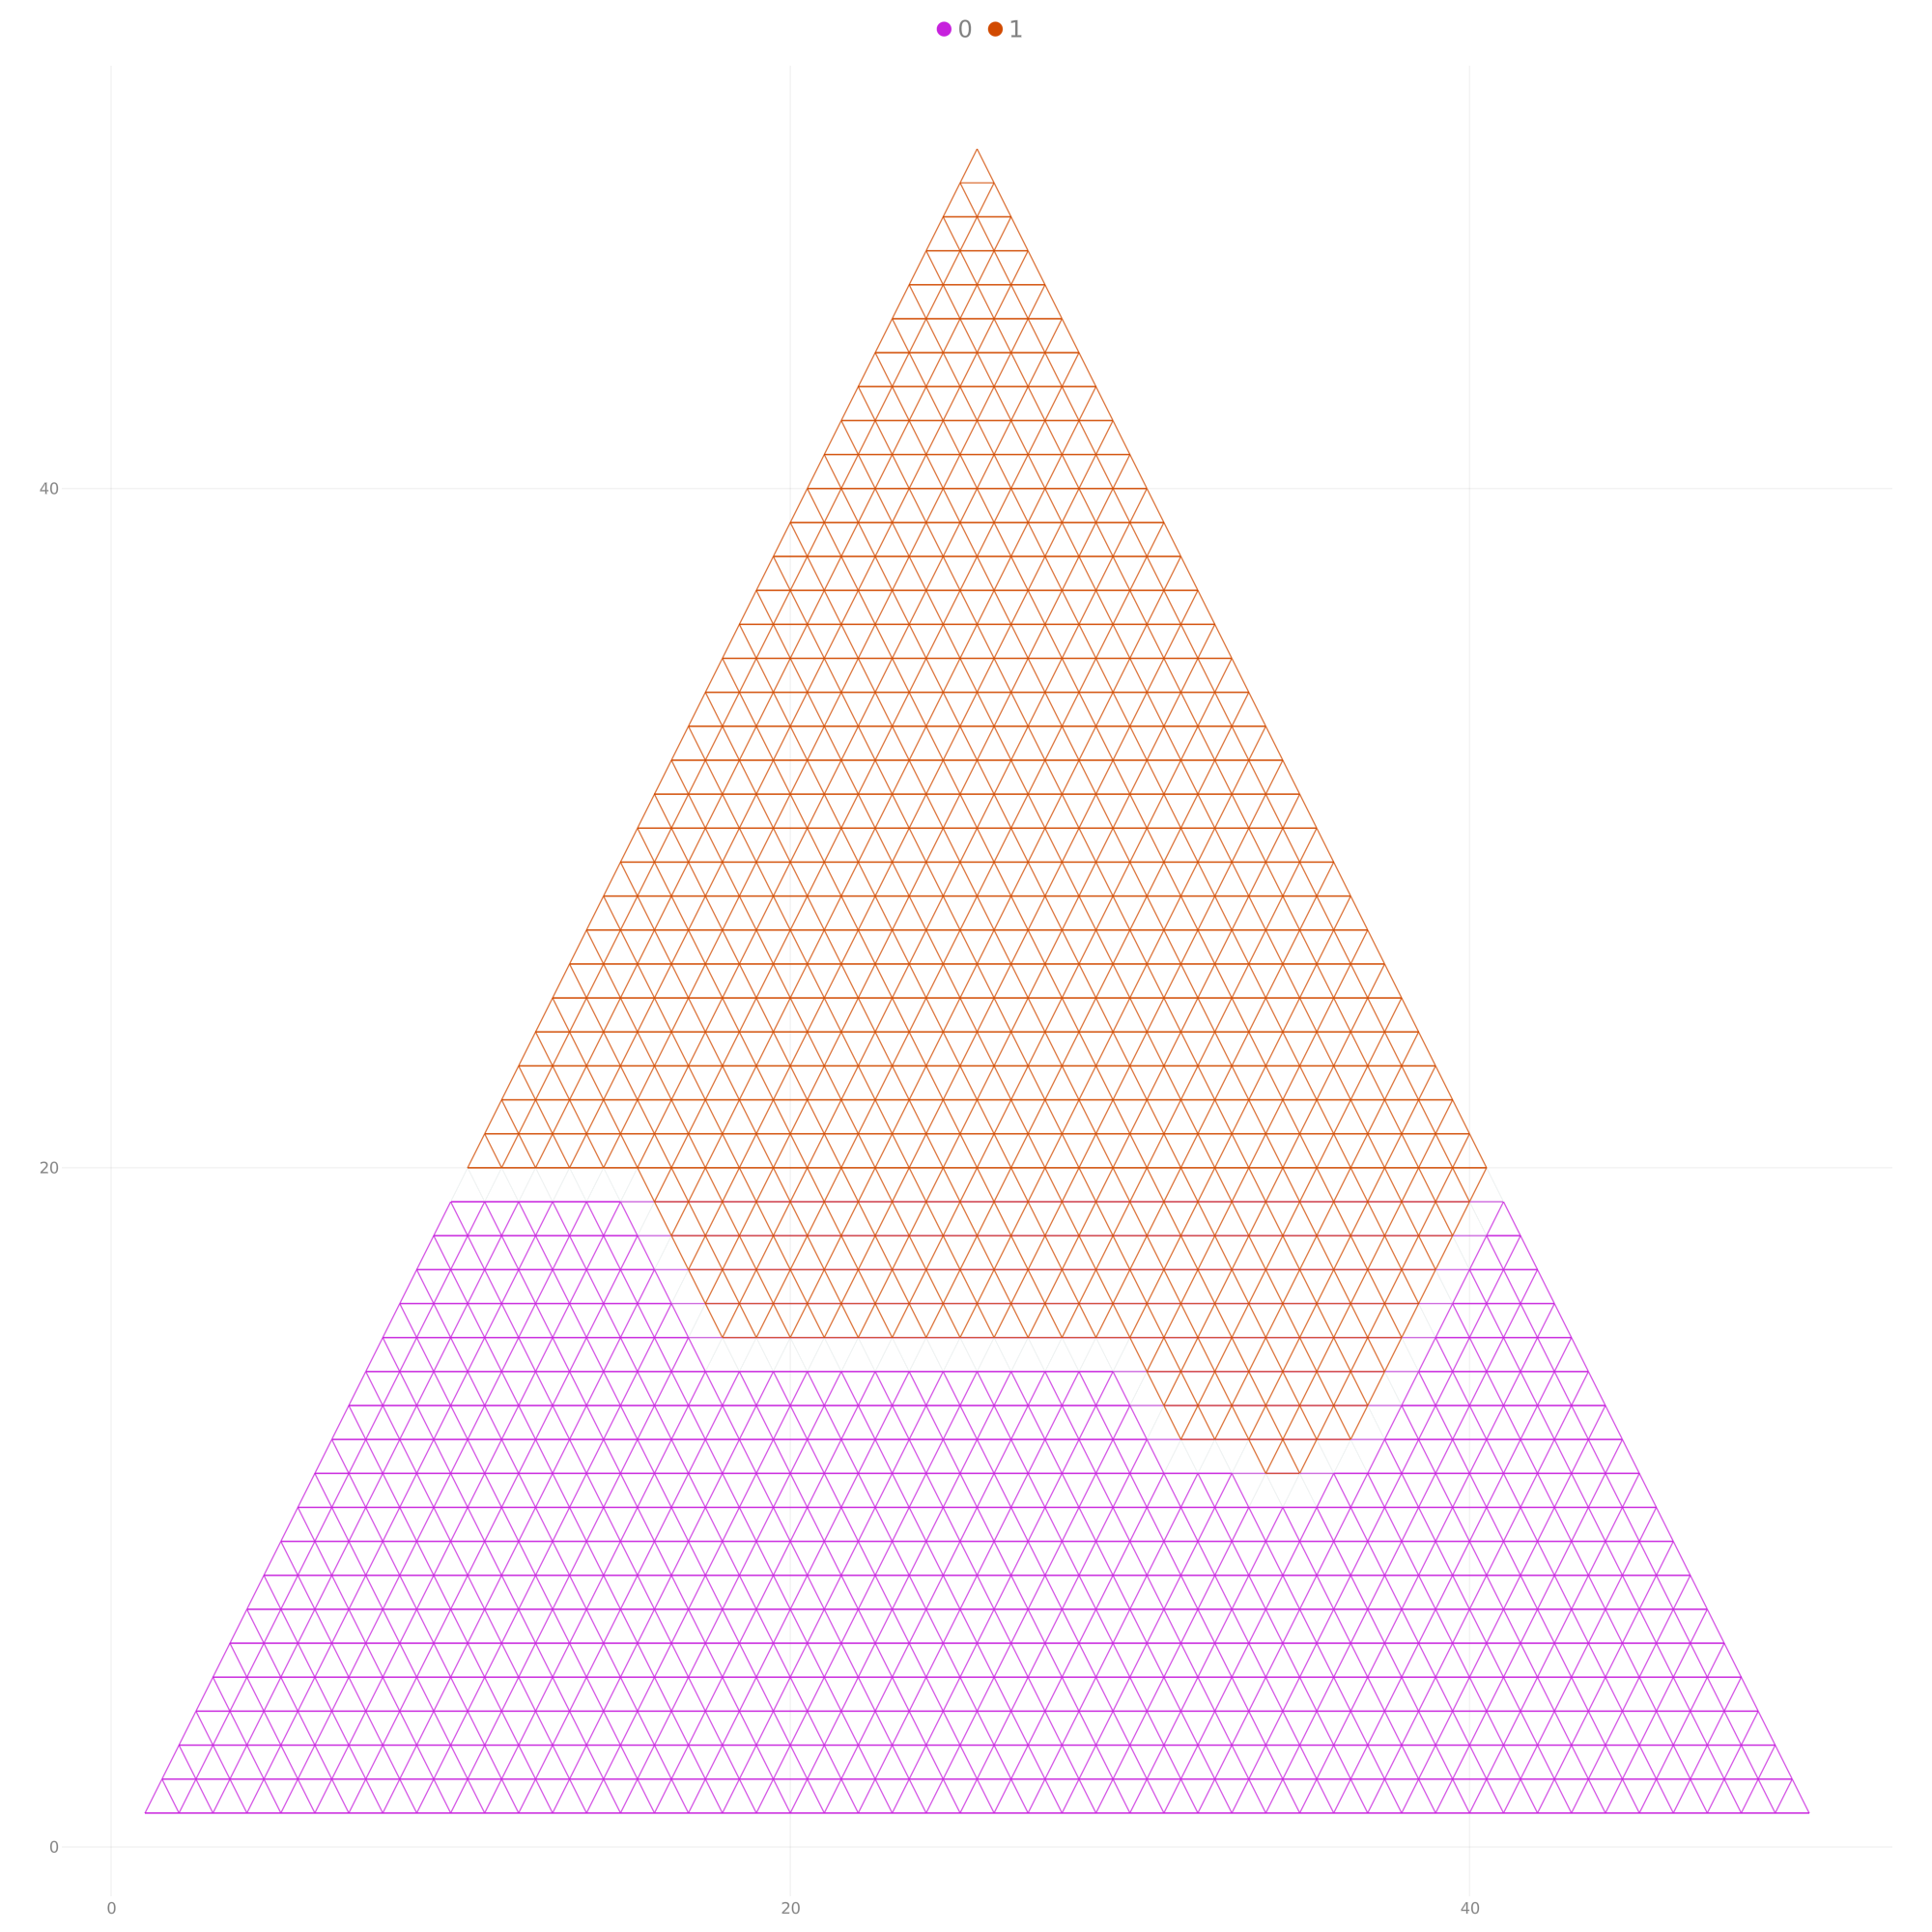
\includegraphics[height=5cm]{fig/plot/bisection/bisection-tapir-metis-cut_80.0}
        \caption{$\texttt {Metis}$ algorithm. \textbf{80 edge cuts}}
    \end{minipage}
        \begin{minipage}{0.5\textwidth}
        \centering
        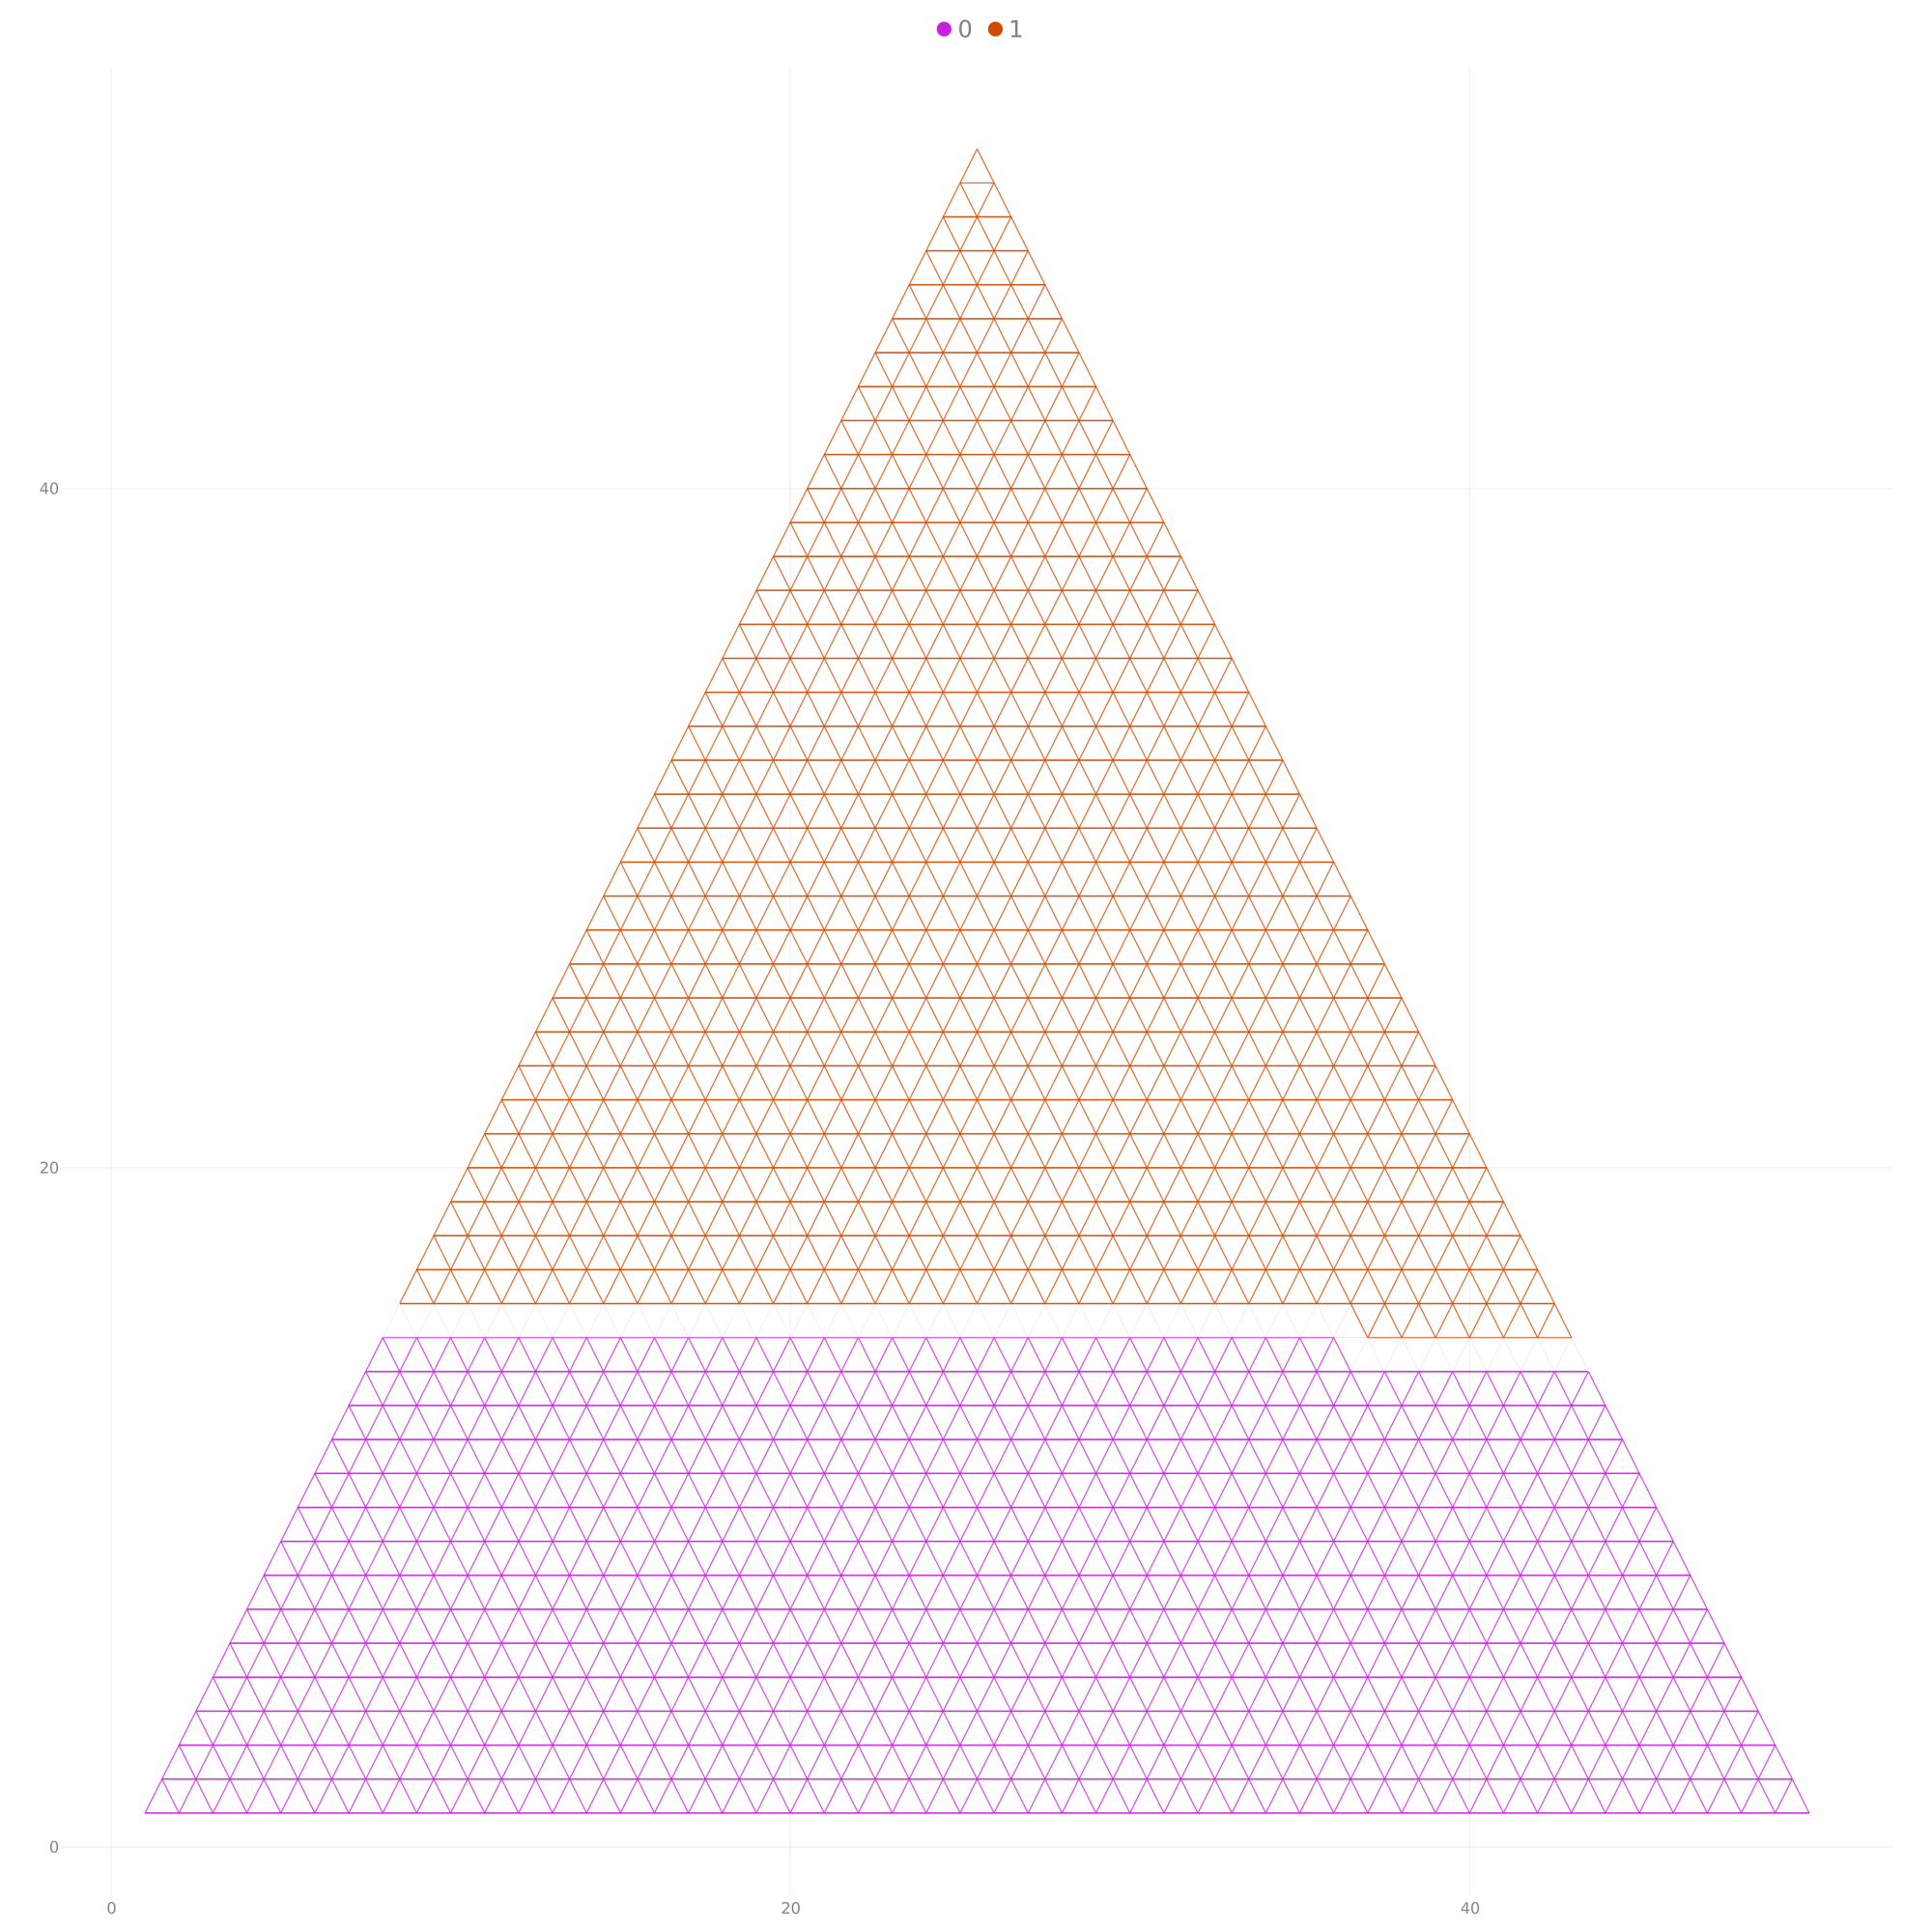
\includegraphics[height=5cm]{fig/plot/bisection/bisection-tapir-inertial-cut_73.0}
        \caption{$\texttt {Inertial}$ algorithm. \textbf{73 edge cuts}}
    \end{minipage}
    \caption*{Partition comparison for mesh $\texttt {tapir}$}
\end{figure}\\
\begin{figure}[h!]
    \begin{minipage}{0.5\textwidth}
        \centering
        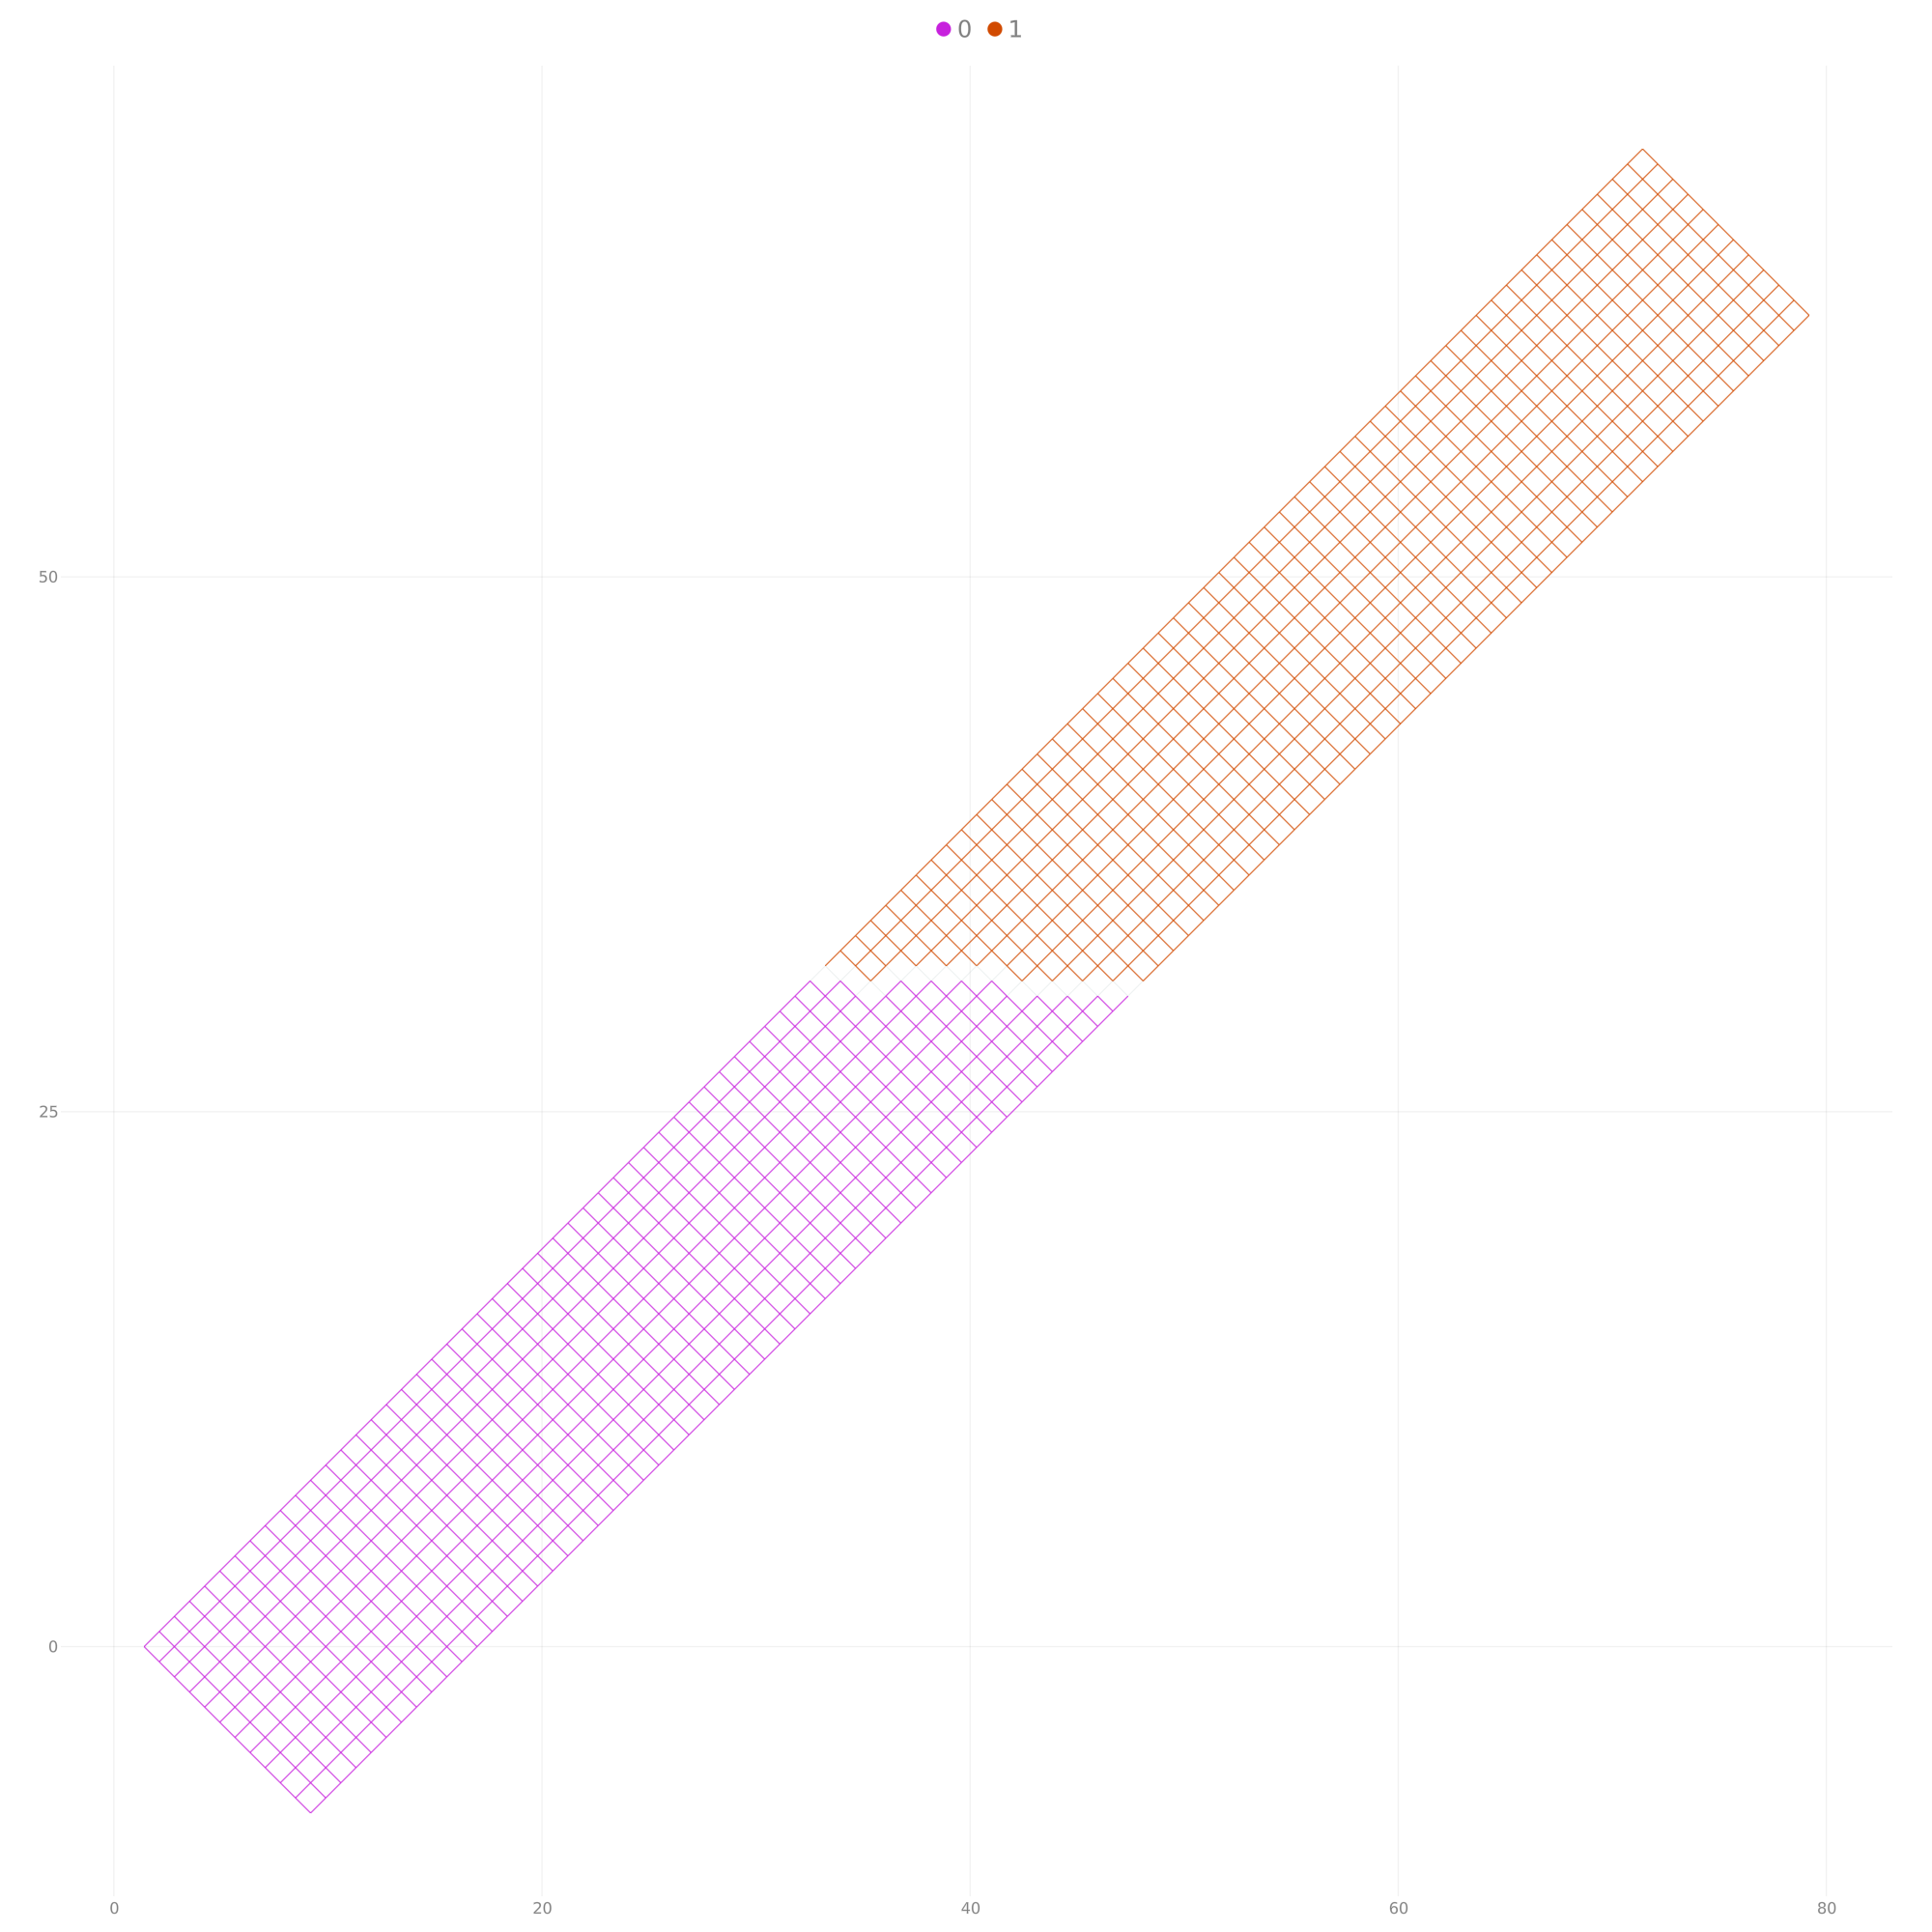
\includegraphics[height=5cm]{fig/plot/bisection/bisection-smallmesh-coordinate-cut_22.0}
        \caption{$\texttt {Coordinate}$ algorithm. \textbf{22 edge cuts}}
    \end{minipage}
        \begin{minipage}{0.5\textwidth}
        \centering
        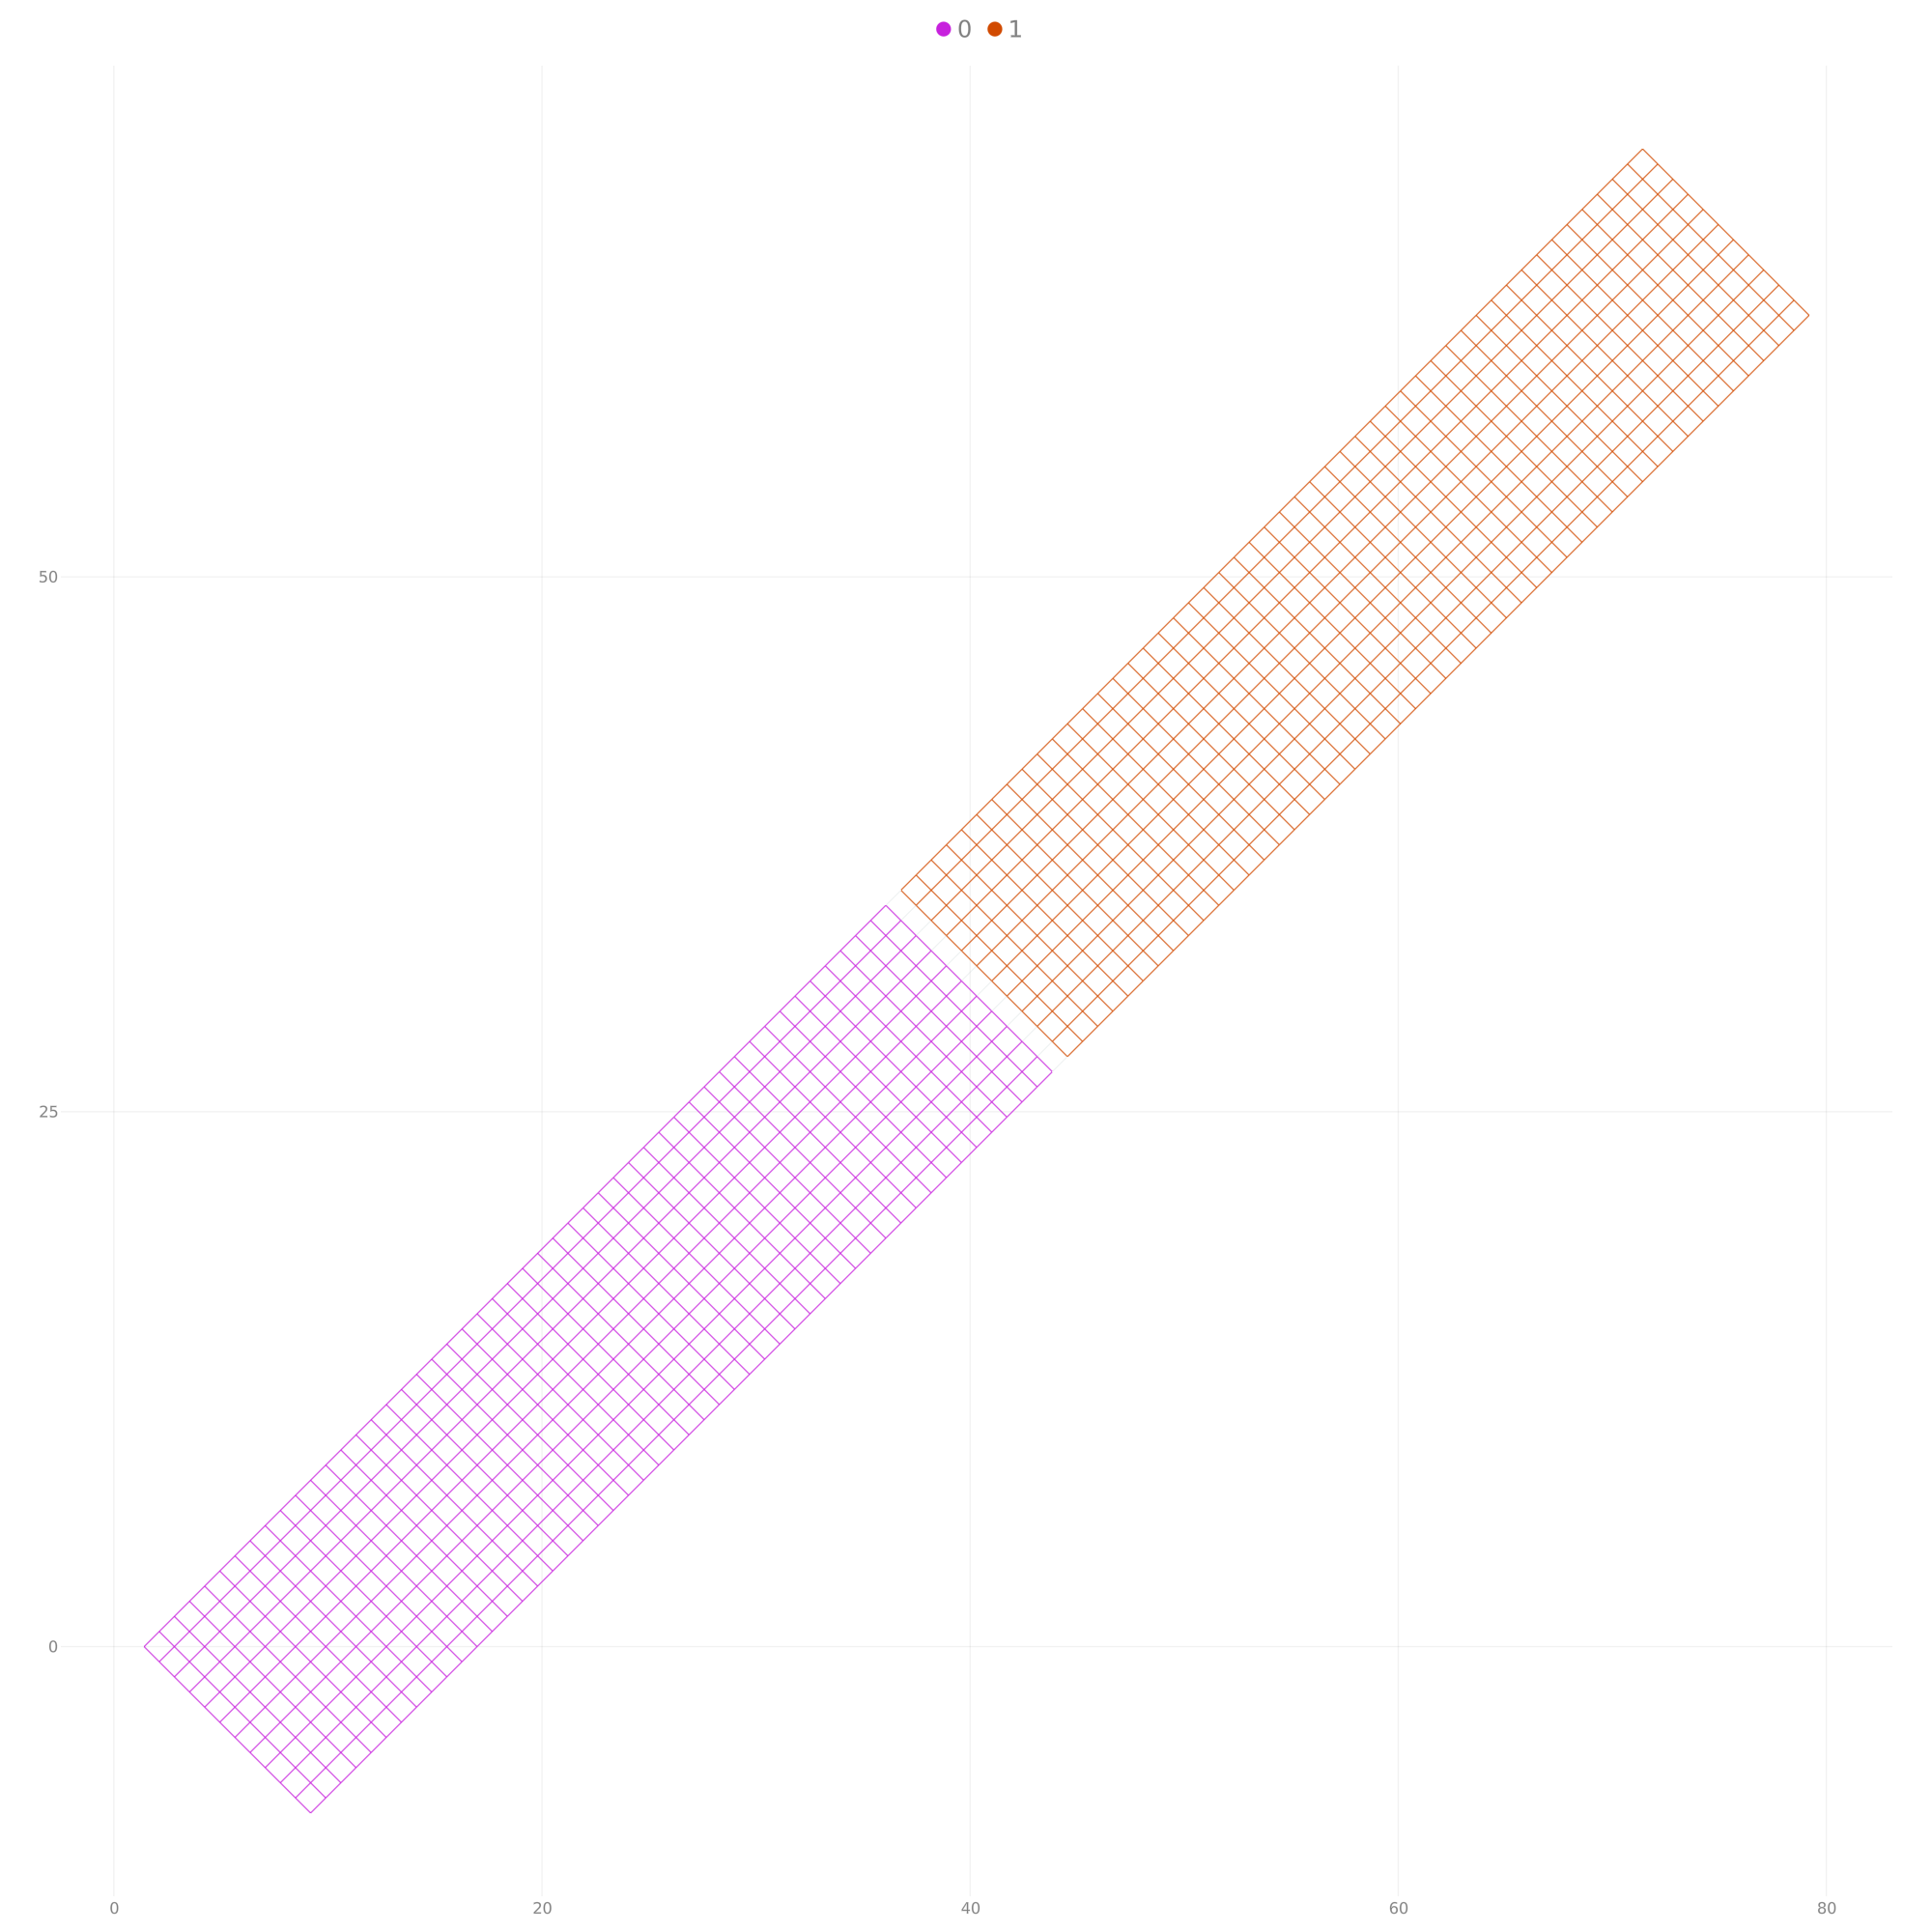
\includegraphics[height=5cm]{fig/plot/bisection/bisection-smallmesh-spectral-cut_12.0}
        \caption{$\texttt {Spectral}$ algorithm. \textbf{12 edge cuts}}
    \end{minipage}
    \caption*{Partition comparison for mesh $\texttt {smallmesh}$}
\end{figure}\\

\clearpage
\subsection{Recursively bisecting meshes [20 points]}
By running the partitioning algorithms recursively, we split each graph/subgraph $G$ into two more subgraphs $G^'$ and $G^{''}$. Using recursion can pay to our advantage if we intend to parallelize and scale our partition computation. \\
We therefore split the graphs into $2^n$ subgraphs where $n$ is the number of recursion levels.\\
One fundamental difference though is that the two partitions that each recursion level yields \textbf{influence all the next recursions}. For $n=3$ and $n=4$ we split the graph into $4$ and $8$ subgraphs respectively.\\
By running the benchmark we notice how the $\texttt {Spectral}$ really stands out for being the affected the most performance-wise from computing the eigenvectors and eigenvalues of very large graphs.\\ Generally, the recursive approach results in greater edge cuts. $\texttt {Inertial}$ yields low edge cuts and is very fast as it always computes eigenvectors of matrix $M\in \mathbb{R}^{2\times 2}$. 

\begin{figure}[h!]
    \begin{minipage}{0.5\textwidth}
        \centering
        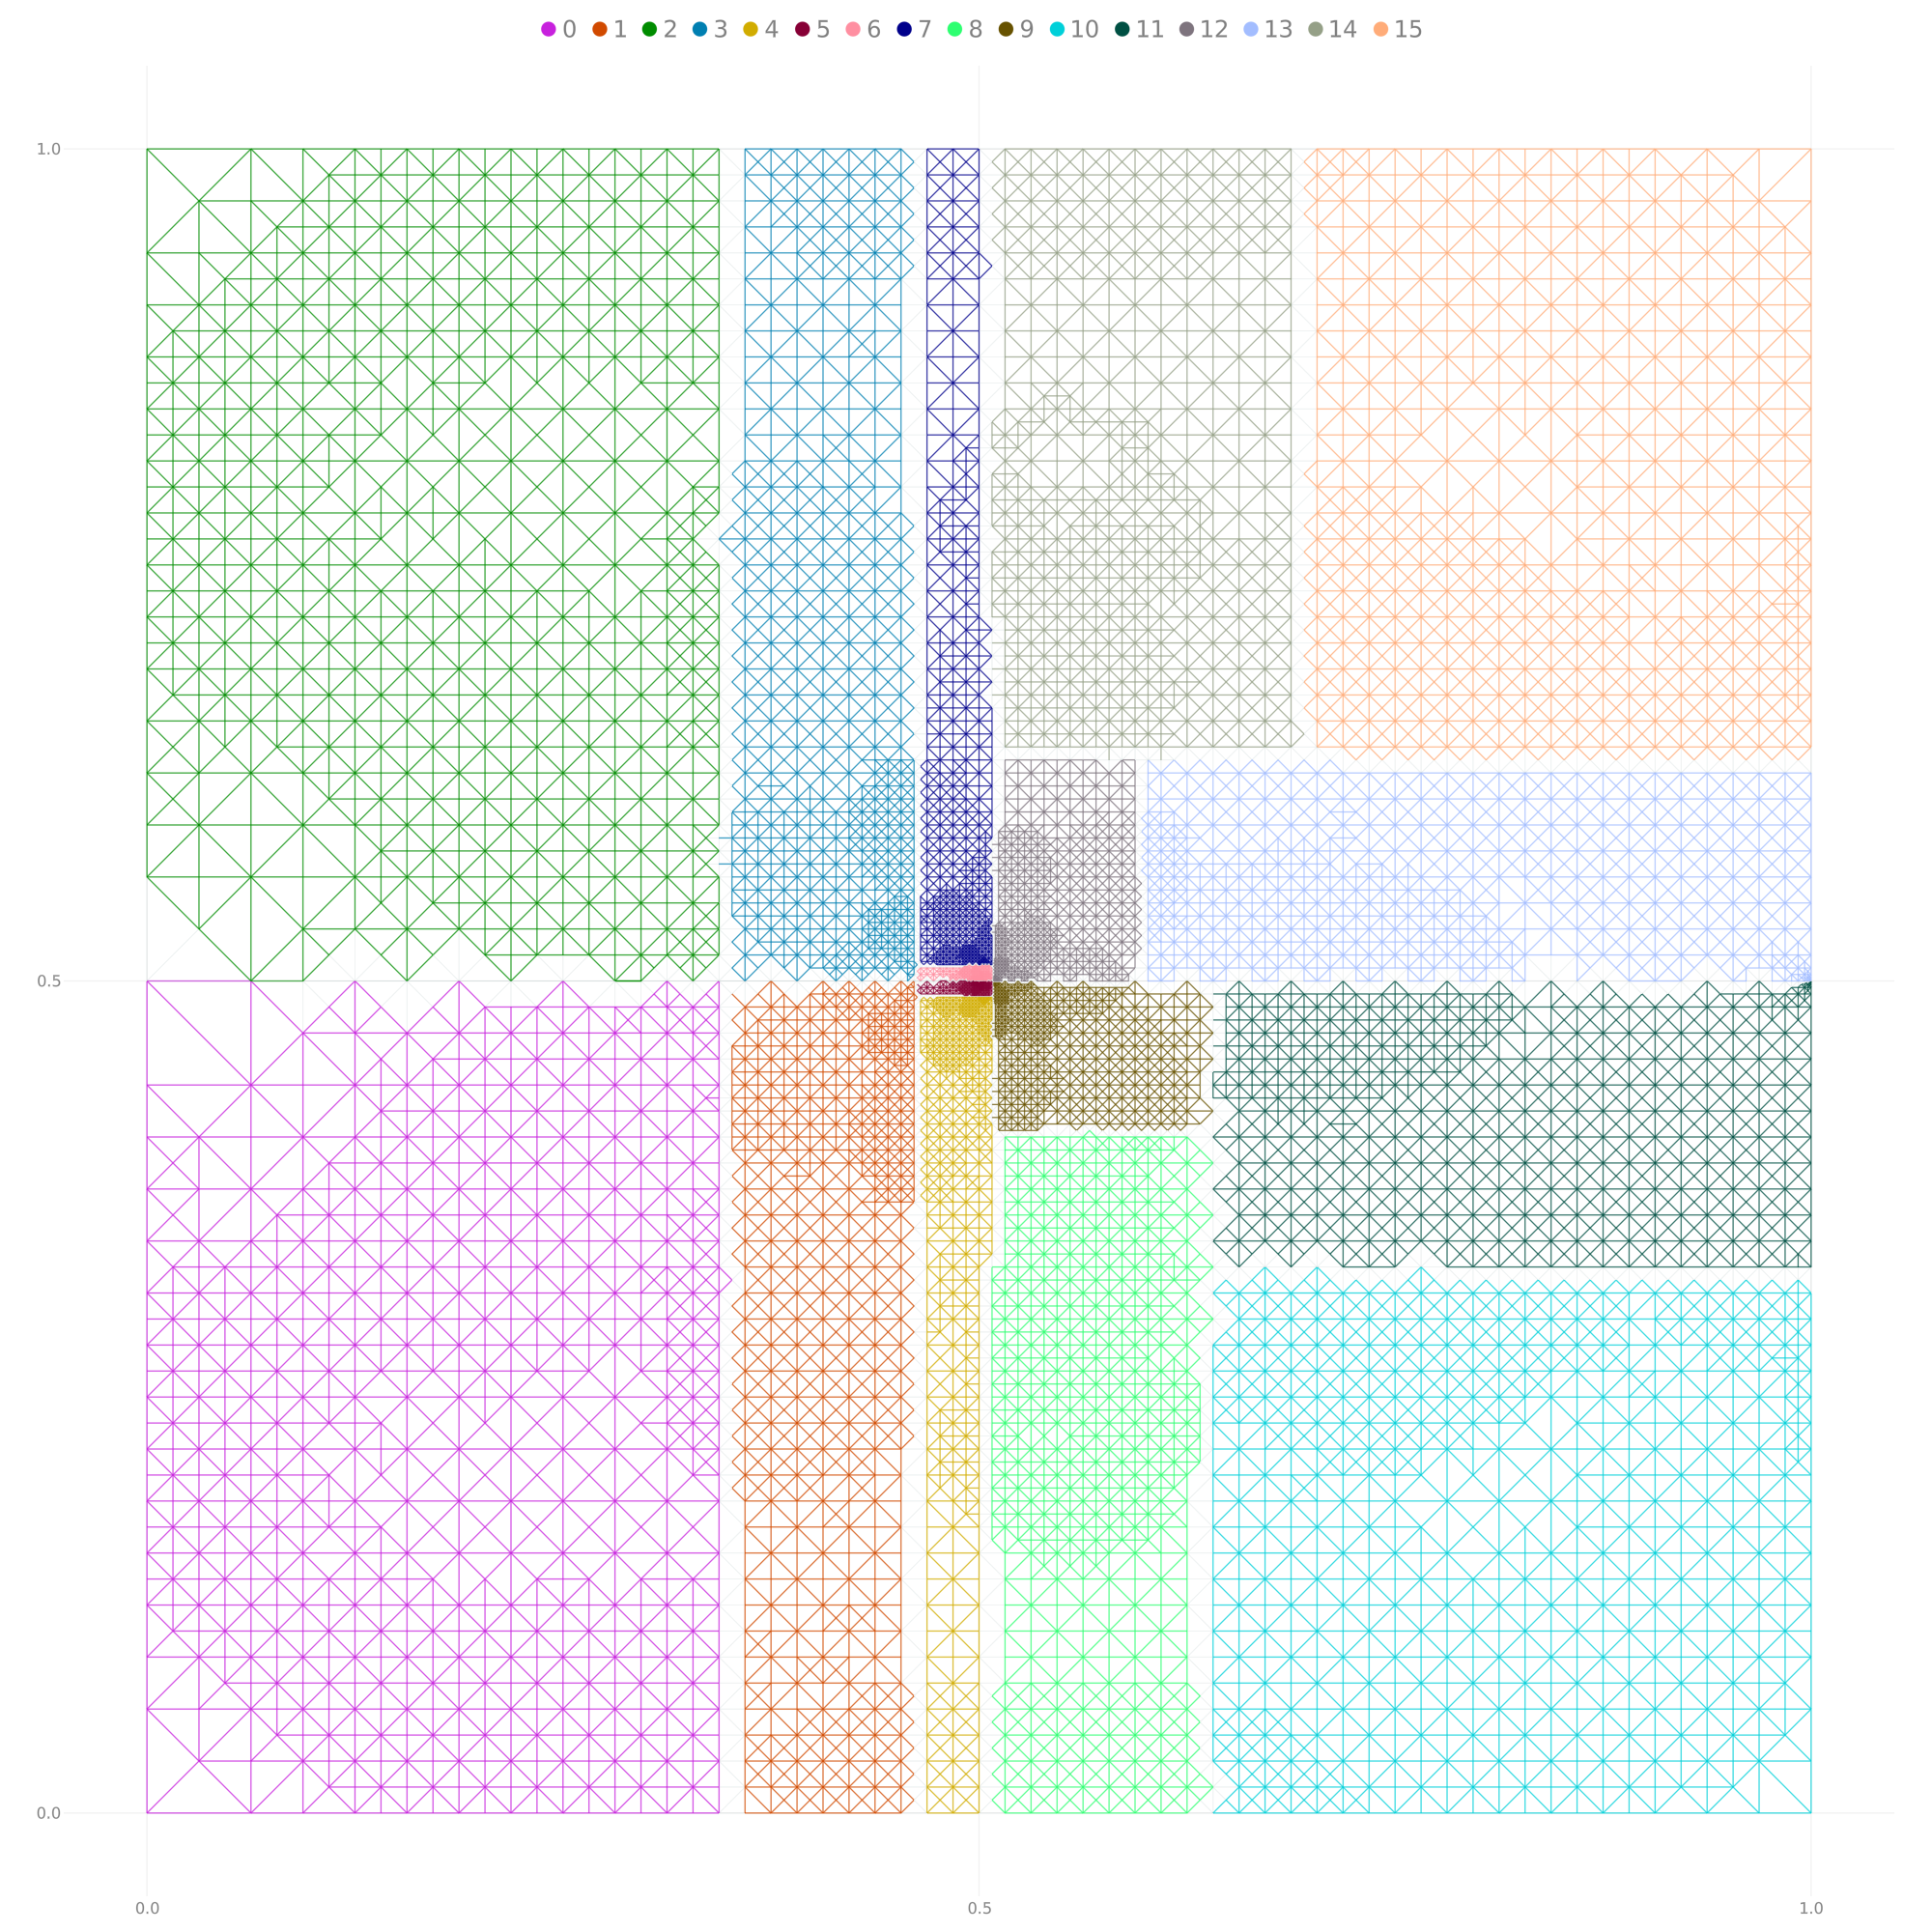
\includegraphics[height=5cm]{fig/plot/recursive/recursive-crack-coordinate-p16-cut_1861.0}
        \caption{$\texttt {Coordinate}$ algorithm.\textbf{1861 edge cuts}}
    \end{minipage}
    \begin{minipage}{0.5\textwidth}
        \centering
        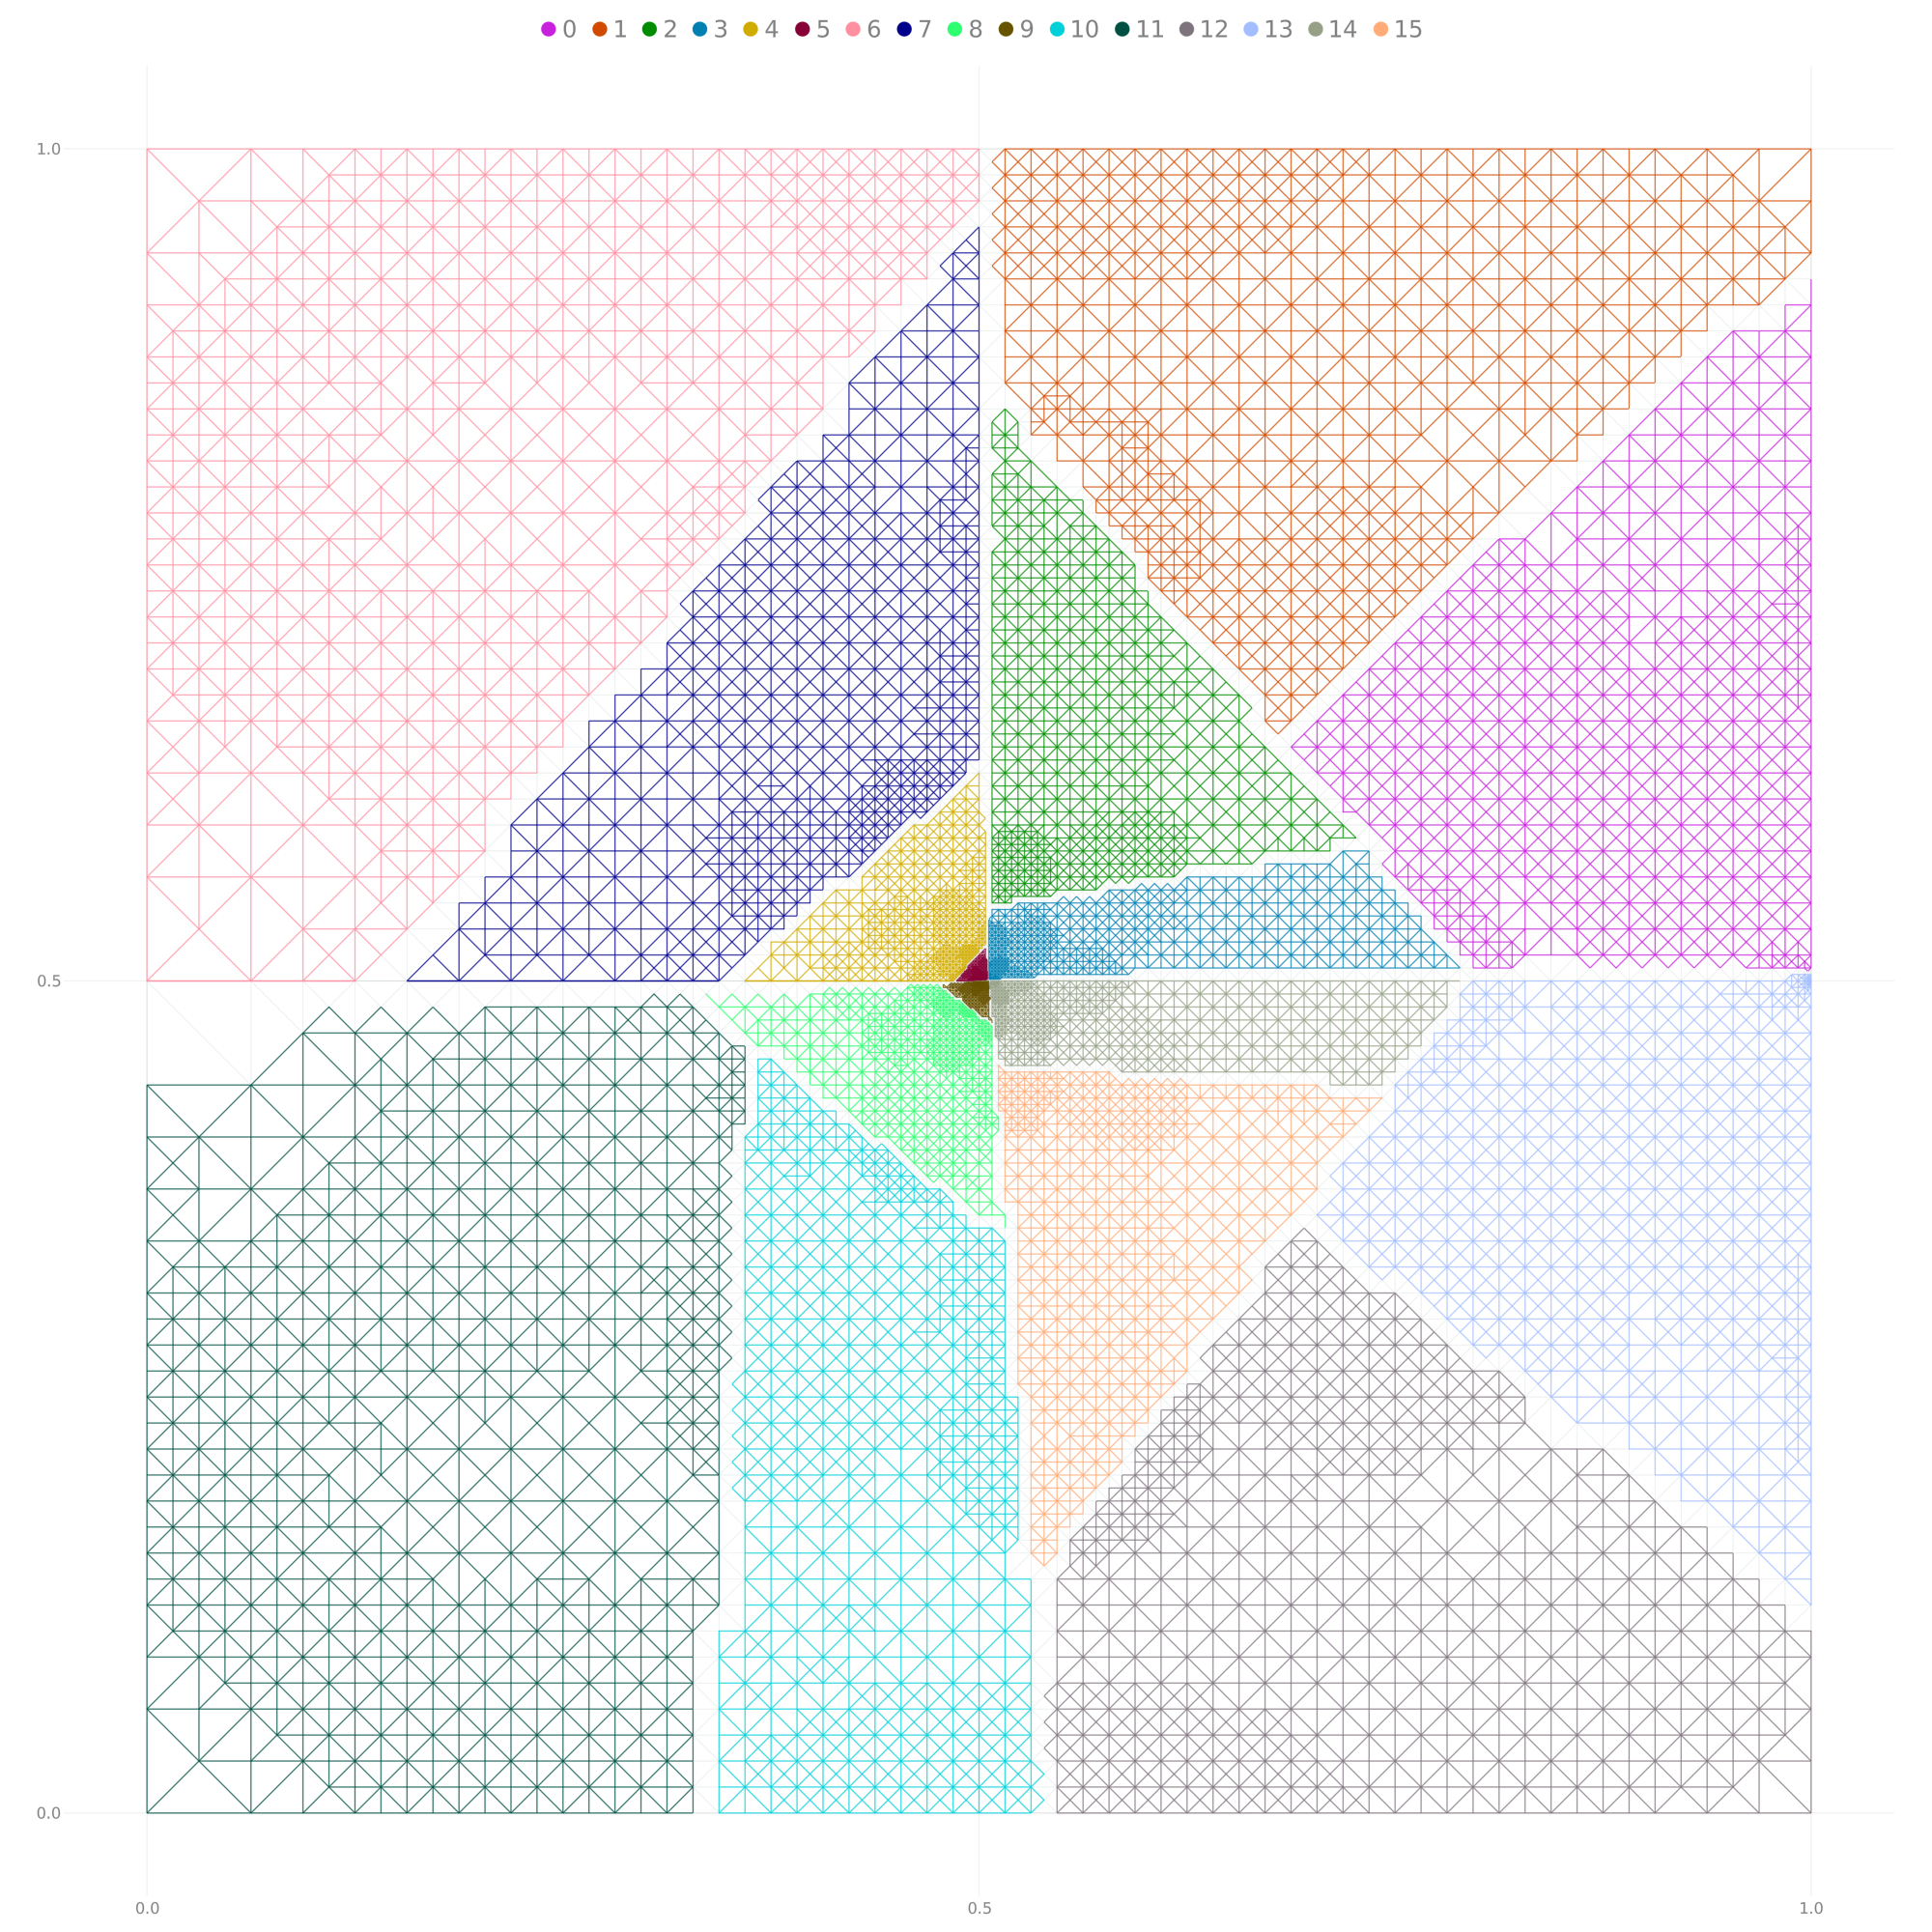
\includegraphics[height=5cm]{fig/plot/recursive/recursive-crack-inertial-p16-cut_1618.0}
        \caption{$\texttt {Inertial}$ algorithm. \textbf{1618 edge cuts}}
    \end{minipage}
        \begin{minipage}{0.5\textwidth}
        \centering
        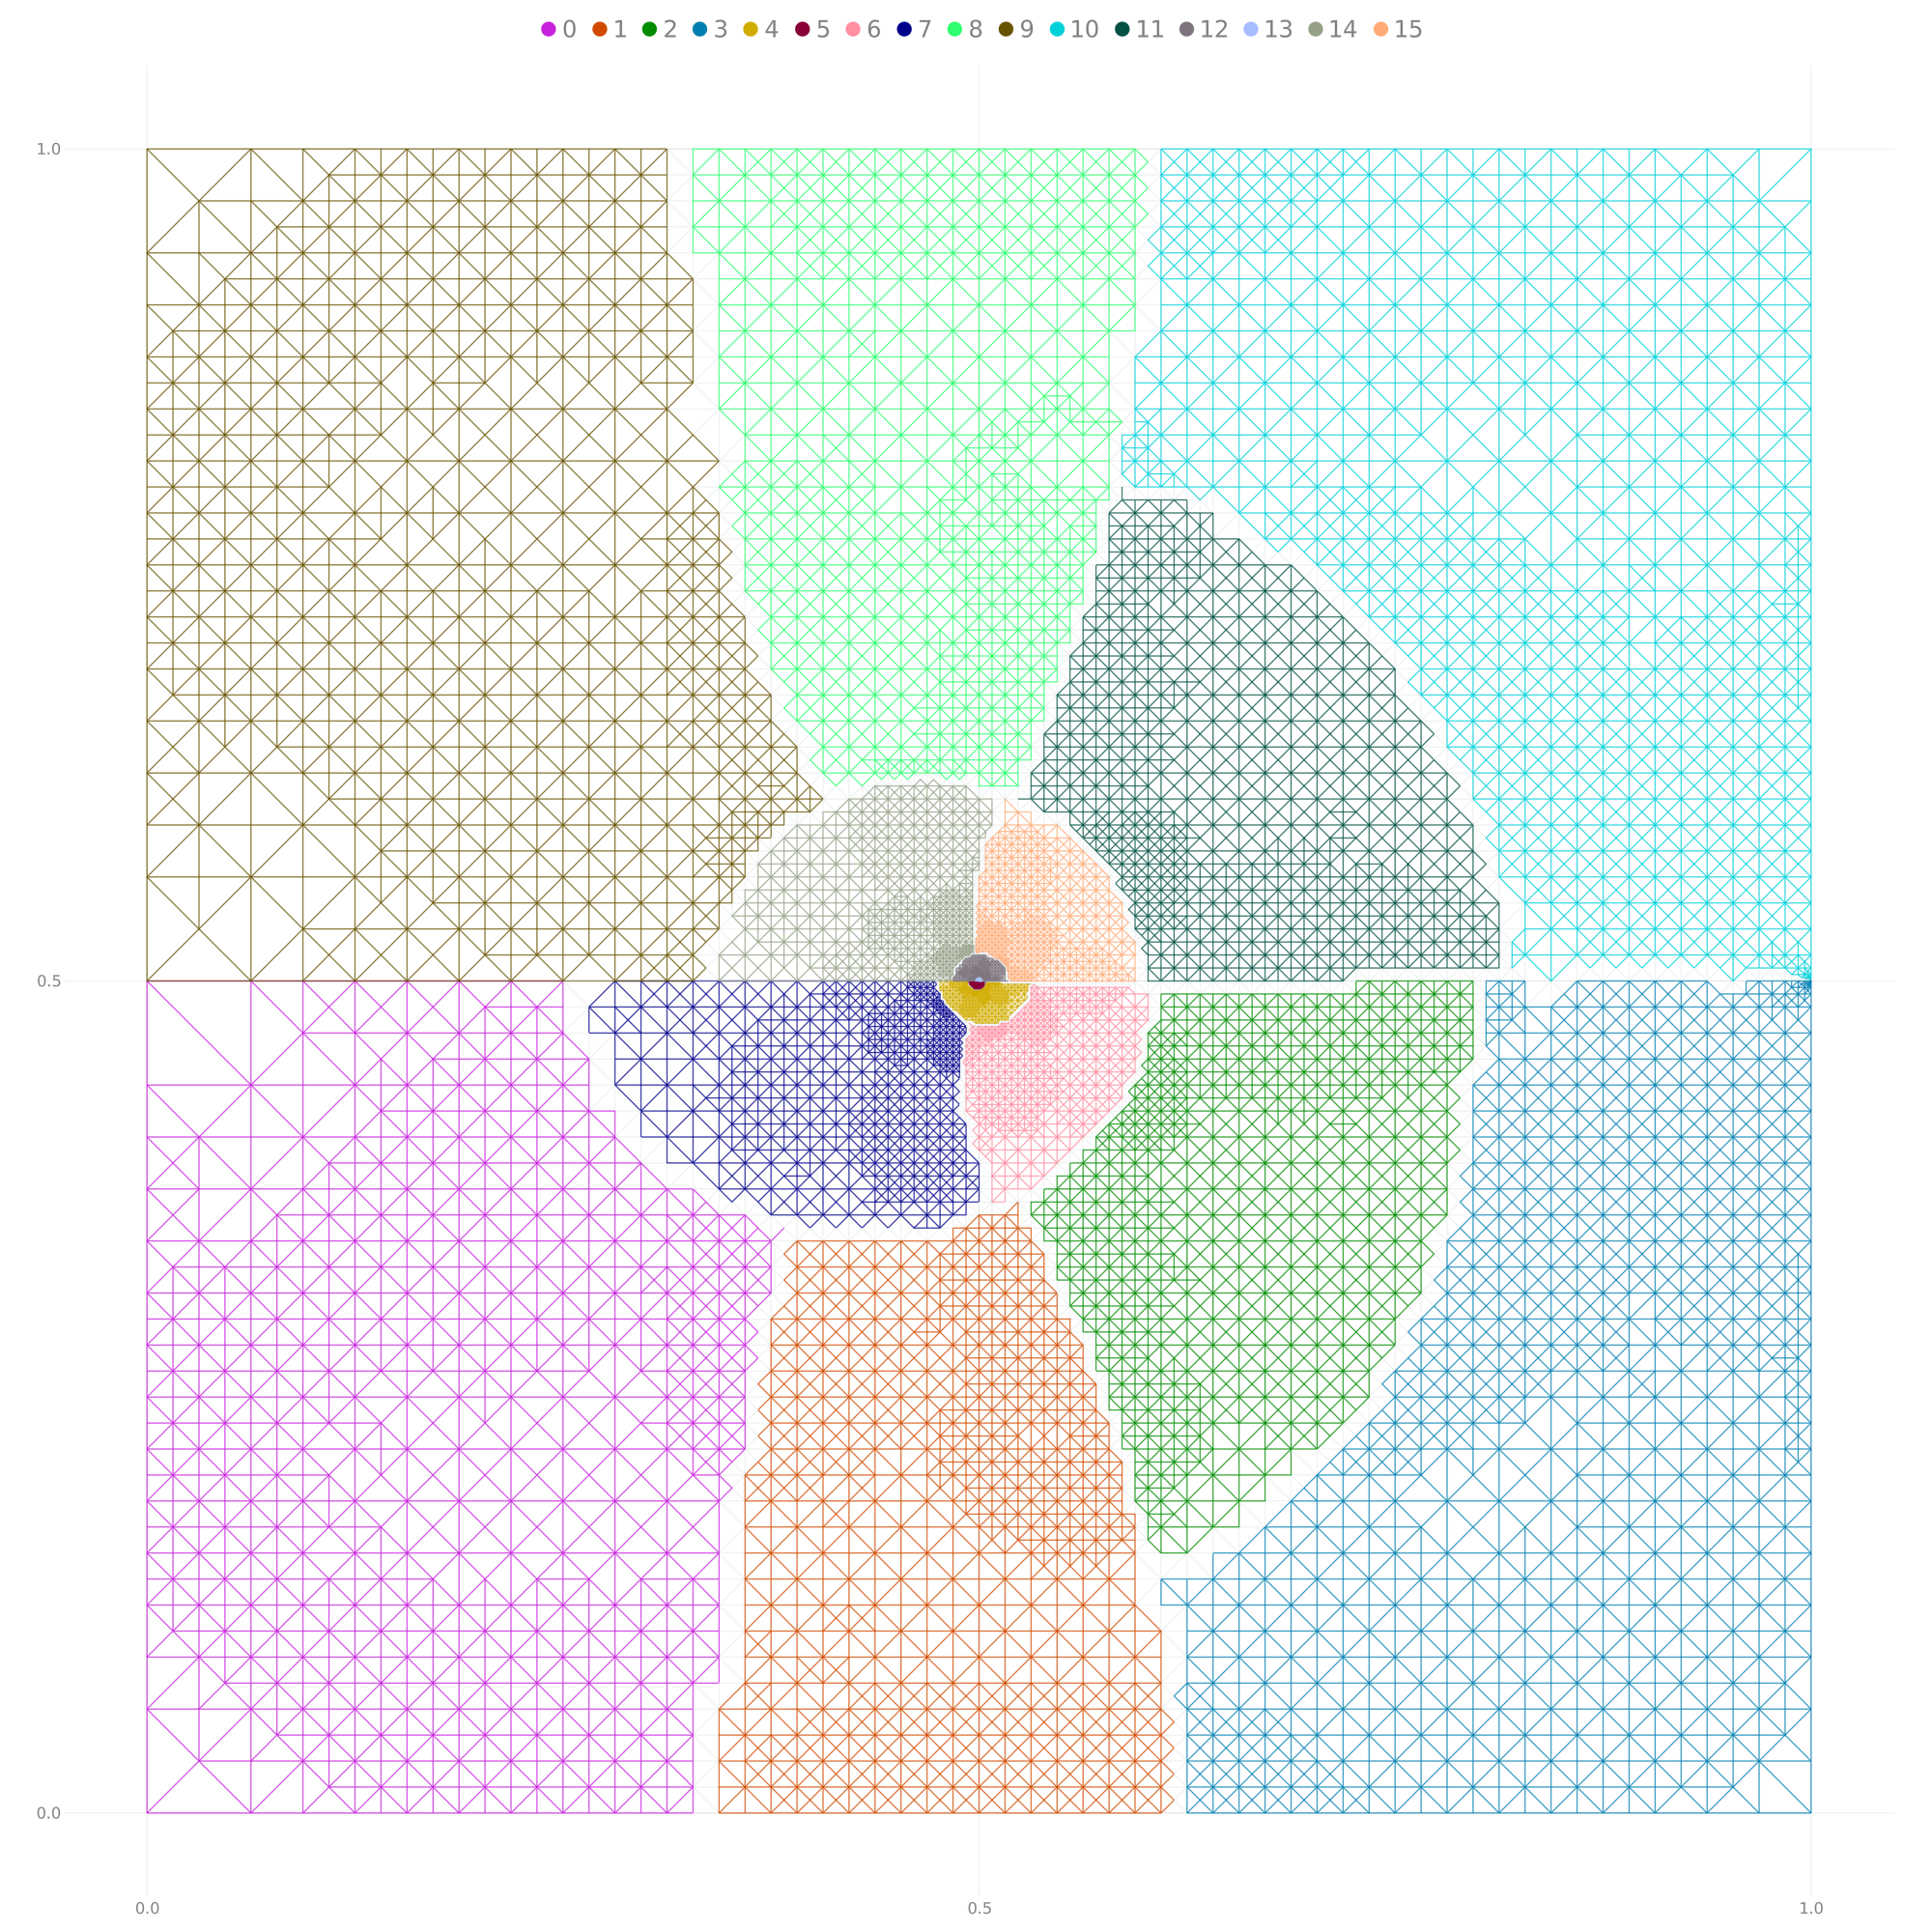
\includegraphics[height=5cm]{fig/plot/recursive/recursive-crack-spectral-p16-cut_1303.0}
        \caption{$\texttt {Spectral}$ algorithm. \textbf{1303 edge cuts}}
    \end{minipage}
    \begin{minipage}{0.5\textwidth}
        \centering
        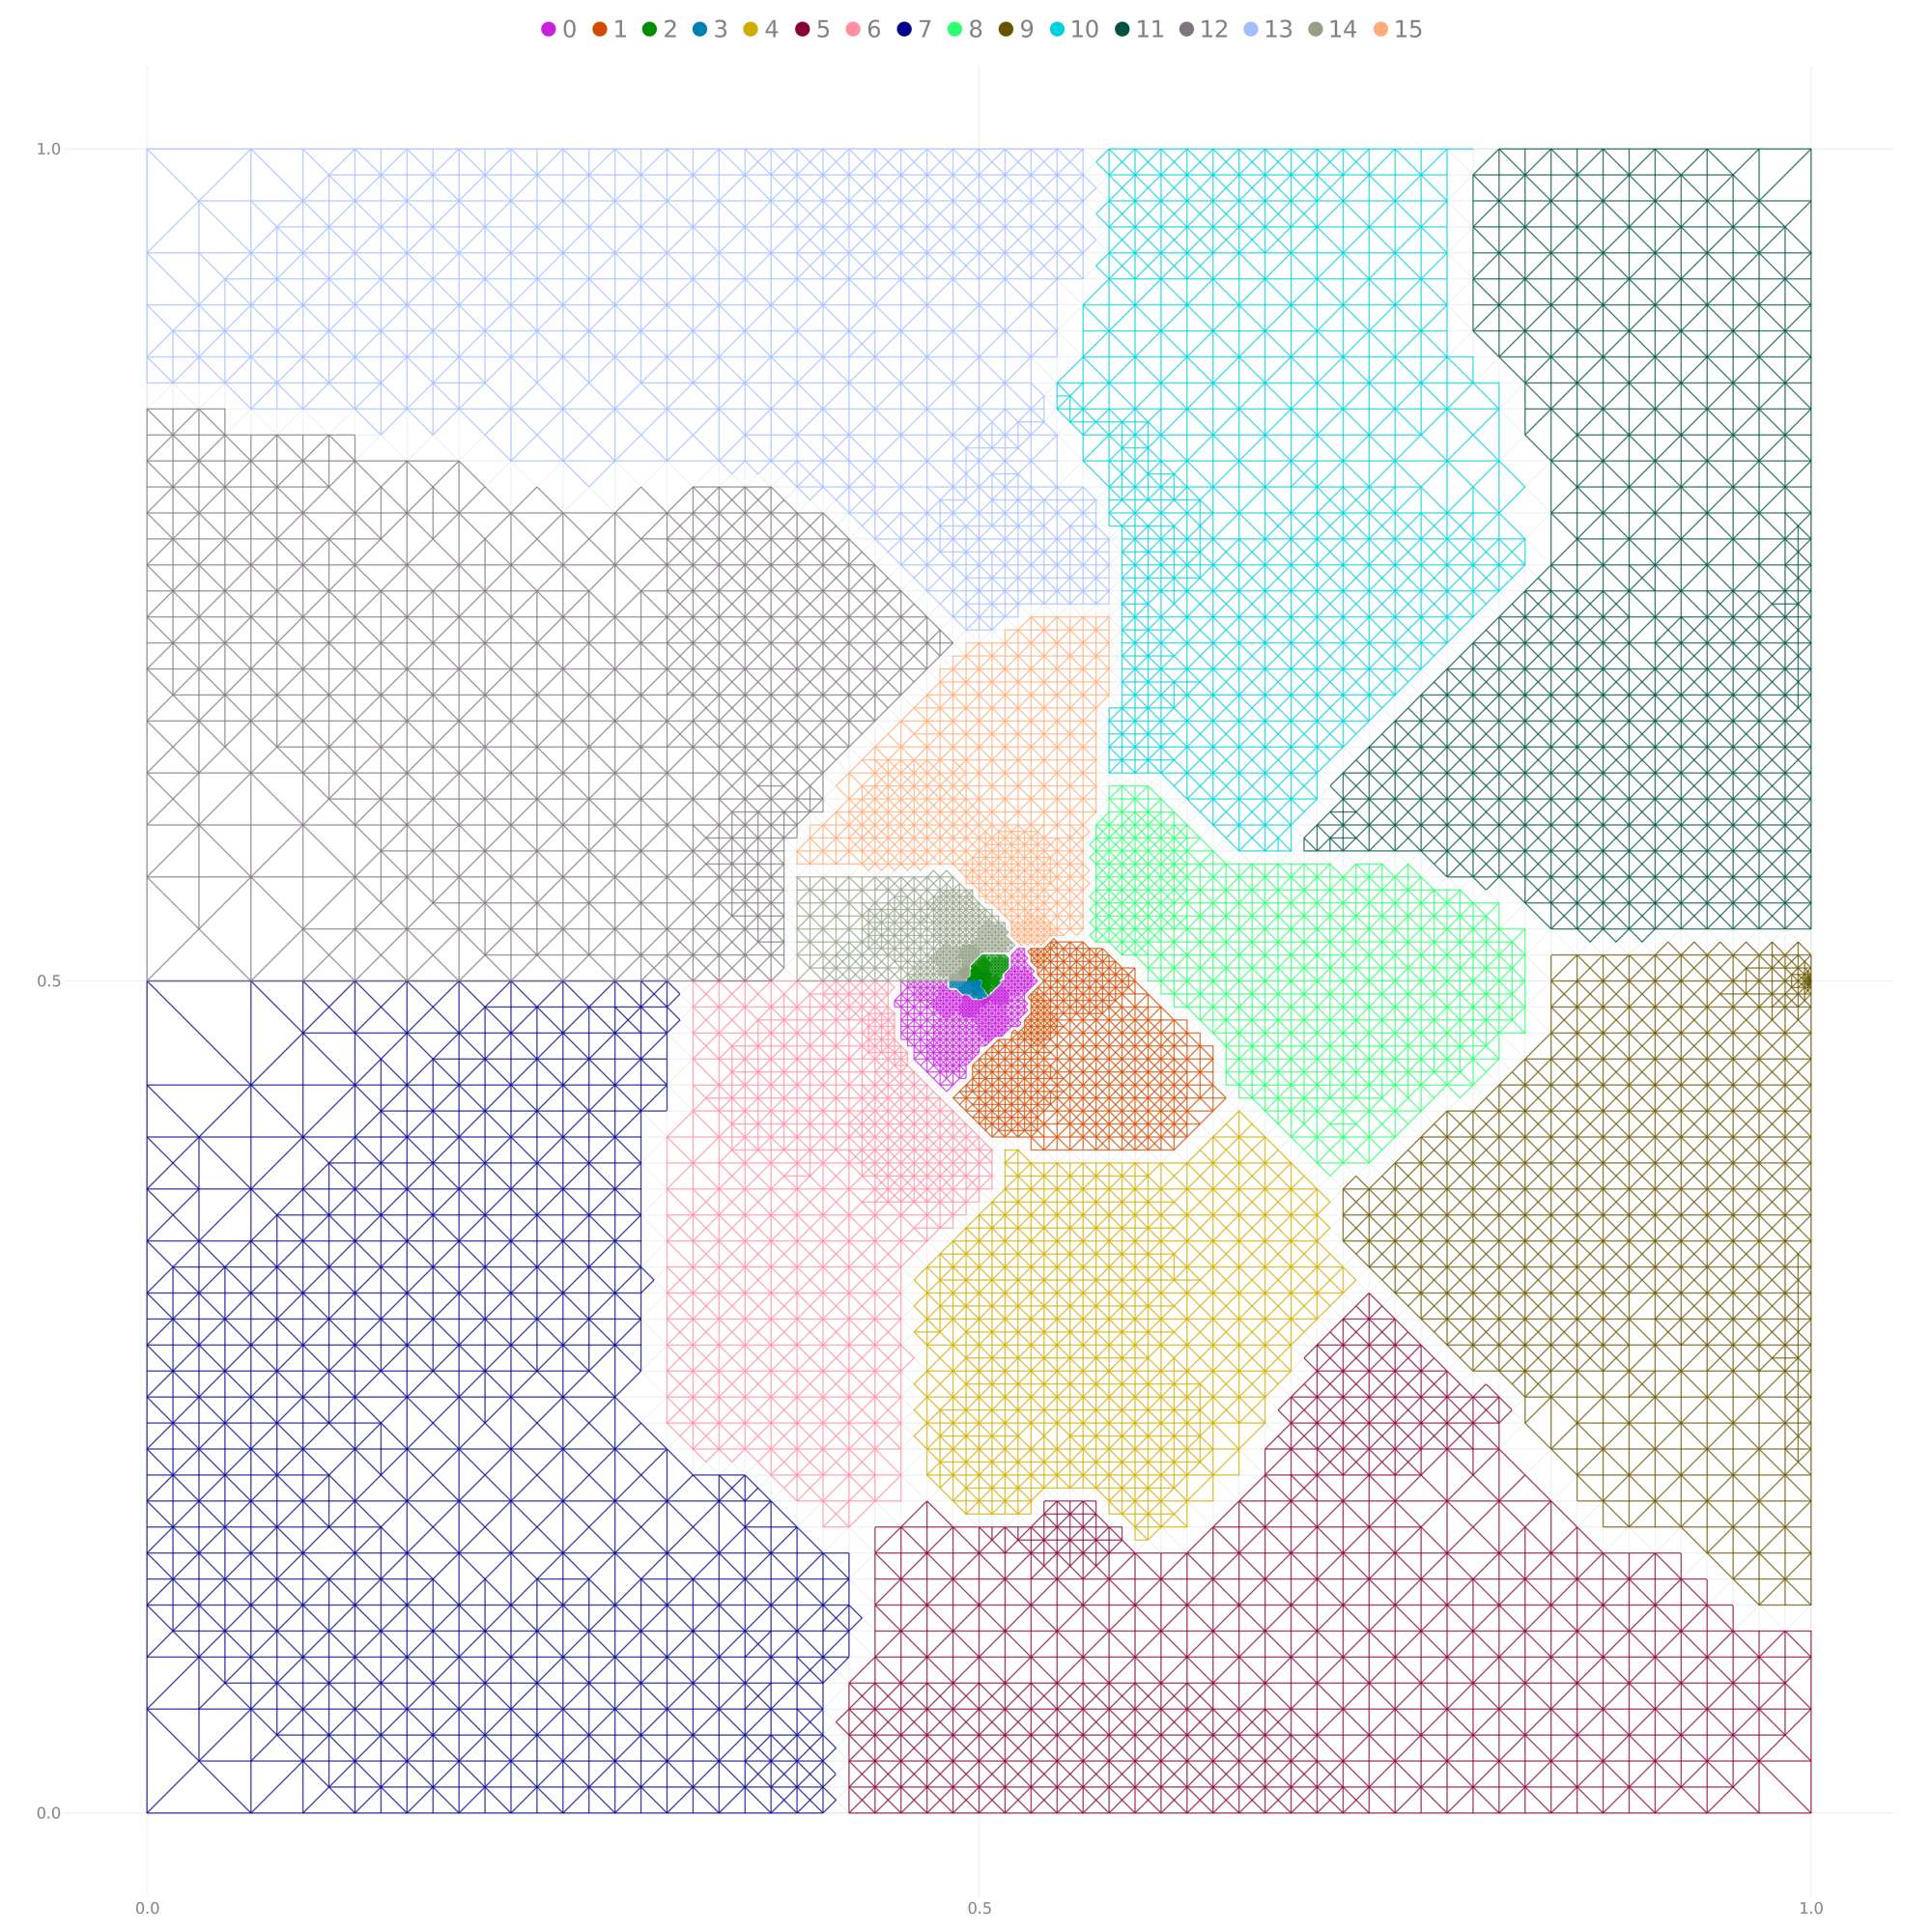
\includegraphics[height=5cm]{fig/plot/recursive/recursive-crack-metis-p16-cut_1276.0}
        \caption{$\texttt {Metis}$ algorithm. \textbf{1276 edge cuts}}
    \end{minipage}
    \caption*{Partition comparison for mesh $\texttt {crack}$ with $n=4$ (16 partitioned subgraphs)}
\end{figure}


\begin{table}[h!]
\caption{Edge-cut results for recursive bi-partitioning.}
\begin{tabular}{l|r|r|r|r|r|r|r|r} \hline\hline 
          Mesh & Spectral & Spectral &   Metis &    Metis & Coordinate & Coordinate & Inertial & Inertial \\
               &  8 parts & 16 parts & 8 parts & 16 parts &    8 parts &   16 parts &  8 parts & 16 parts \\
\hline
      airfoil1 &    327.0 &    578.0 &   311.0 &    580.0 &      516.0 &      819.0 &    578.0 &    904.0 \\
 netz4504\_dual &    105.0 &    174.0 &   100.0 &    154.0 &      127.0 &      198.0 &    122.0 &    202.0 \\
         stufe &    124.0 &    216.0 &   112.0 &    197.0 &      123.0 &      228.0 &    135.0 &    268.0 \\
          3elt &    372.0 &    671.0 &   418.0 &    651.0 &      733.0 &     1168.0 &    880.0 &   1342.0 \\
        barth4 &    505.0 &    758.0 &   491.0 &    773.0 &      875.0 &     1306.0 &    892.0 &   1350.0 \\
       ukerbe1 &    118.0 &    224.0 &   125.0 &    241.0 &      225.0 &      374.0 &    280.0 &    469.0 \\
         crack &    804.0 &   1303.0 &   759.0 &   1276.0 &     1344.0 &     1861.0 &   1061.0 &   1618.0 \\


 \hline \hline
\end{tabular}
\label{table:Rec_bisection}
\end{table}

\clearpage
\subsection{Comparing recursive bisection to direct $k$-way partitioning [15 points]}
Running the $\texttt bench_recursive.jl$ yields the following results.\\
In our case we notice that our count of edge cuts is almost double in larger graphs when partitioning in $32$ subgraphs, either with $k\texttt {-way}$ or recursive partitioning.
\begin{figure}[h!]
    \begin{minipage}{0.5\textwidth}
        \centering
        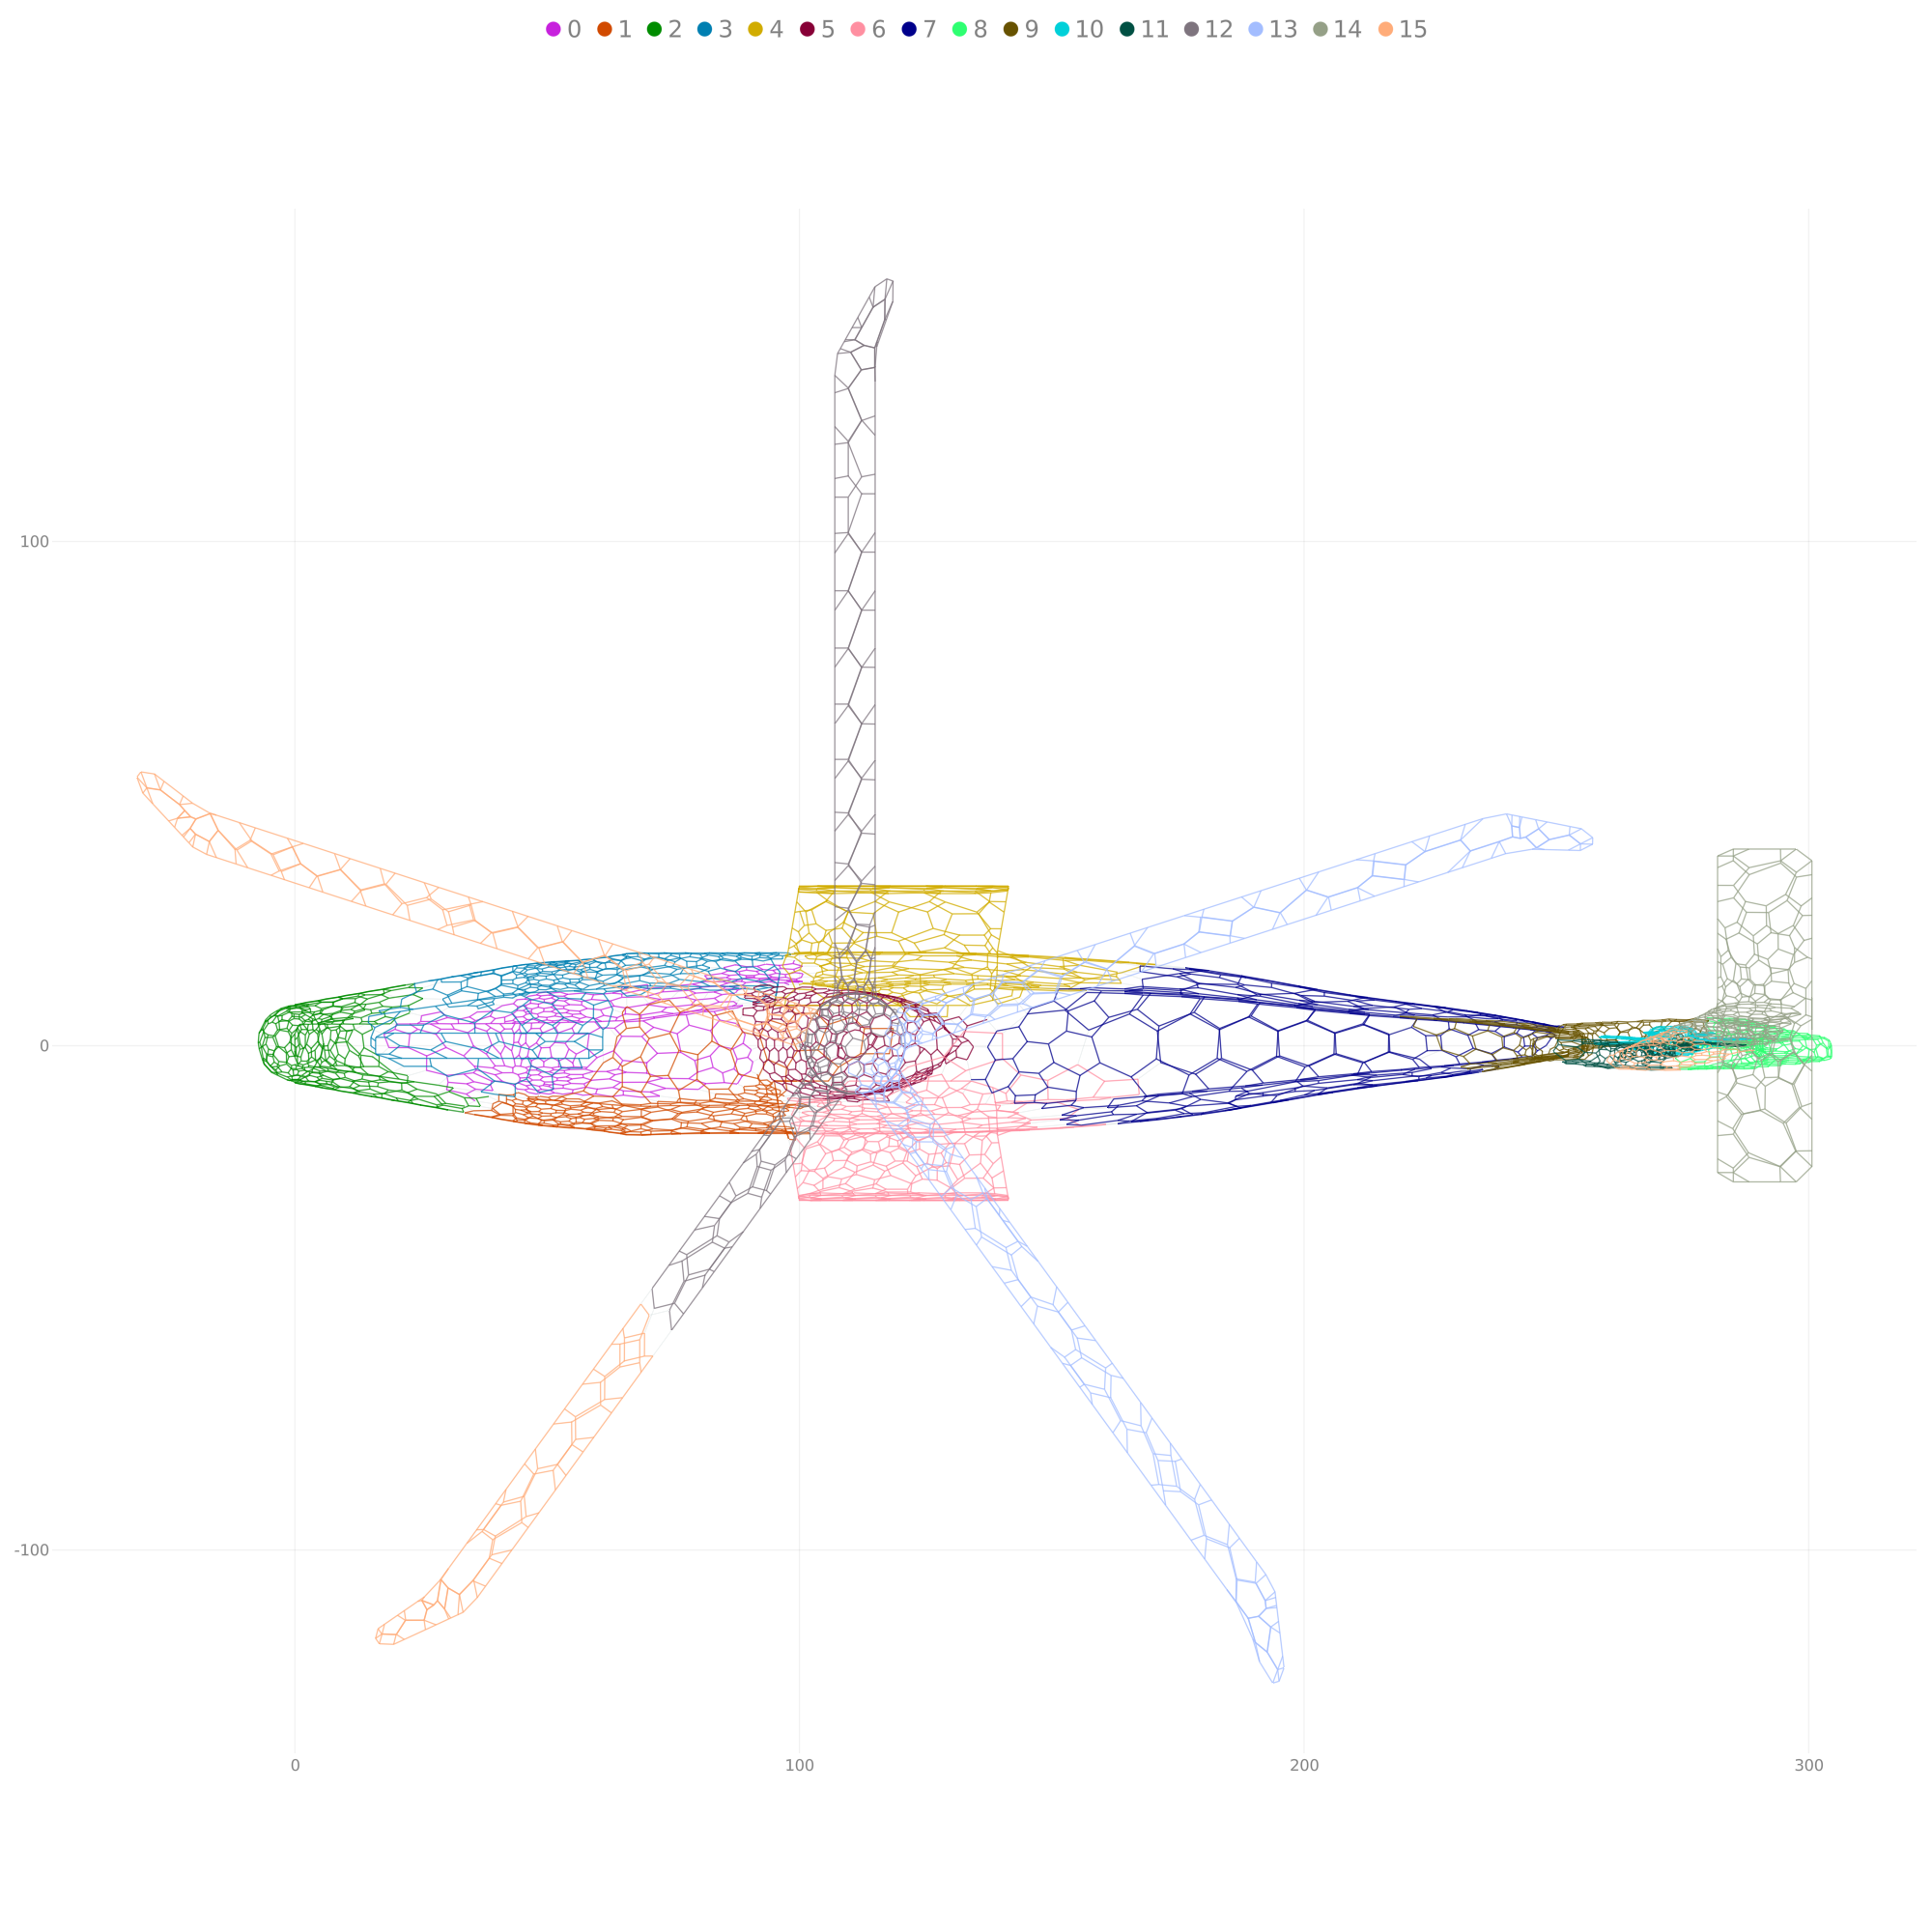
\includegraphics[height=5cm]{fig/plot/metis/metis-commanche_dual-kway-p16-cut_336.0.png}
        \caption{$k$-way partitioning.\\\textbf{336 edge cuts}}
    \end{minipage}
    \begin{minipage}{0.5\textwidth}
        \centering
        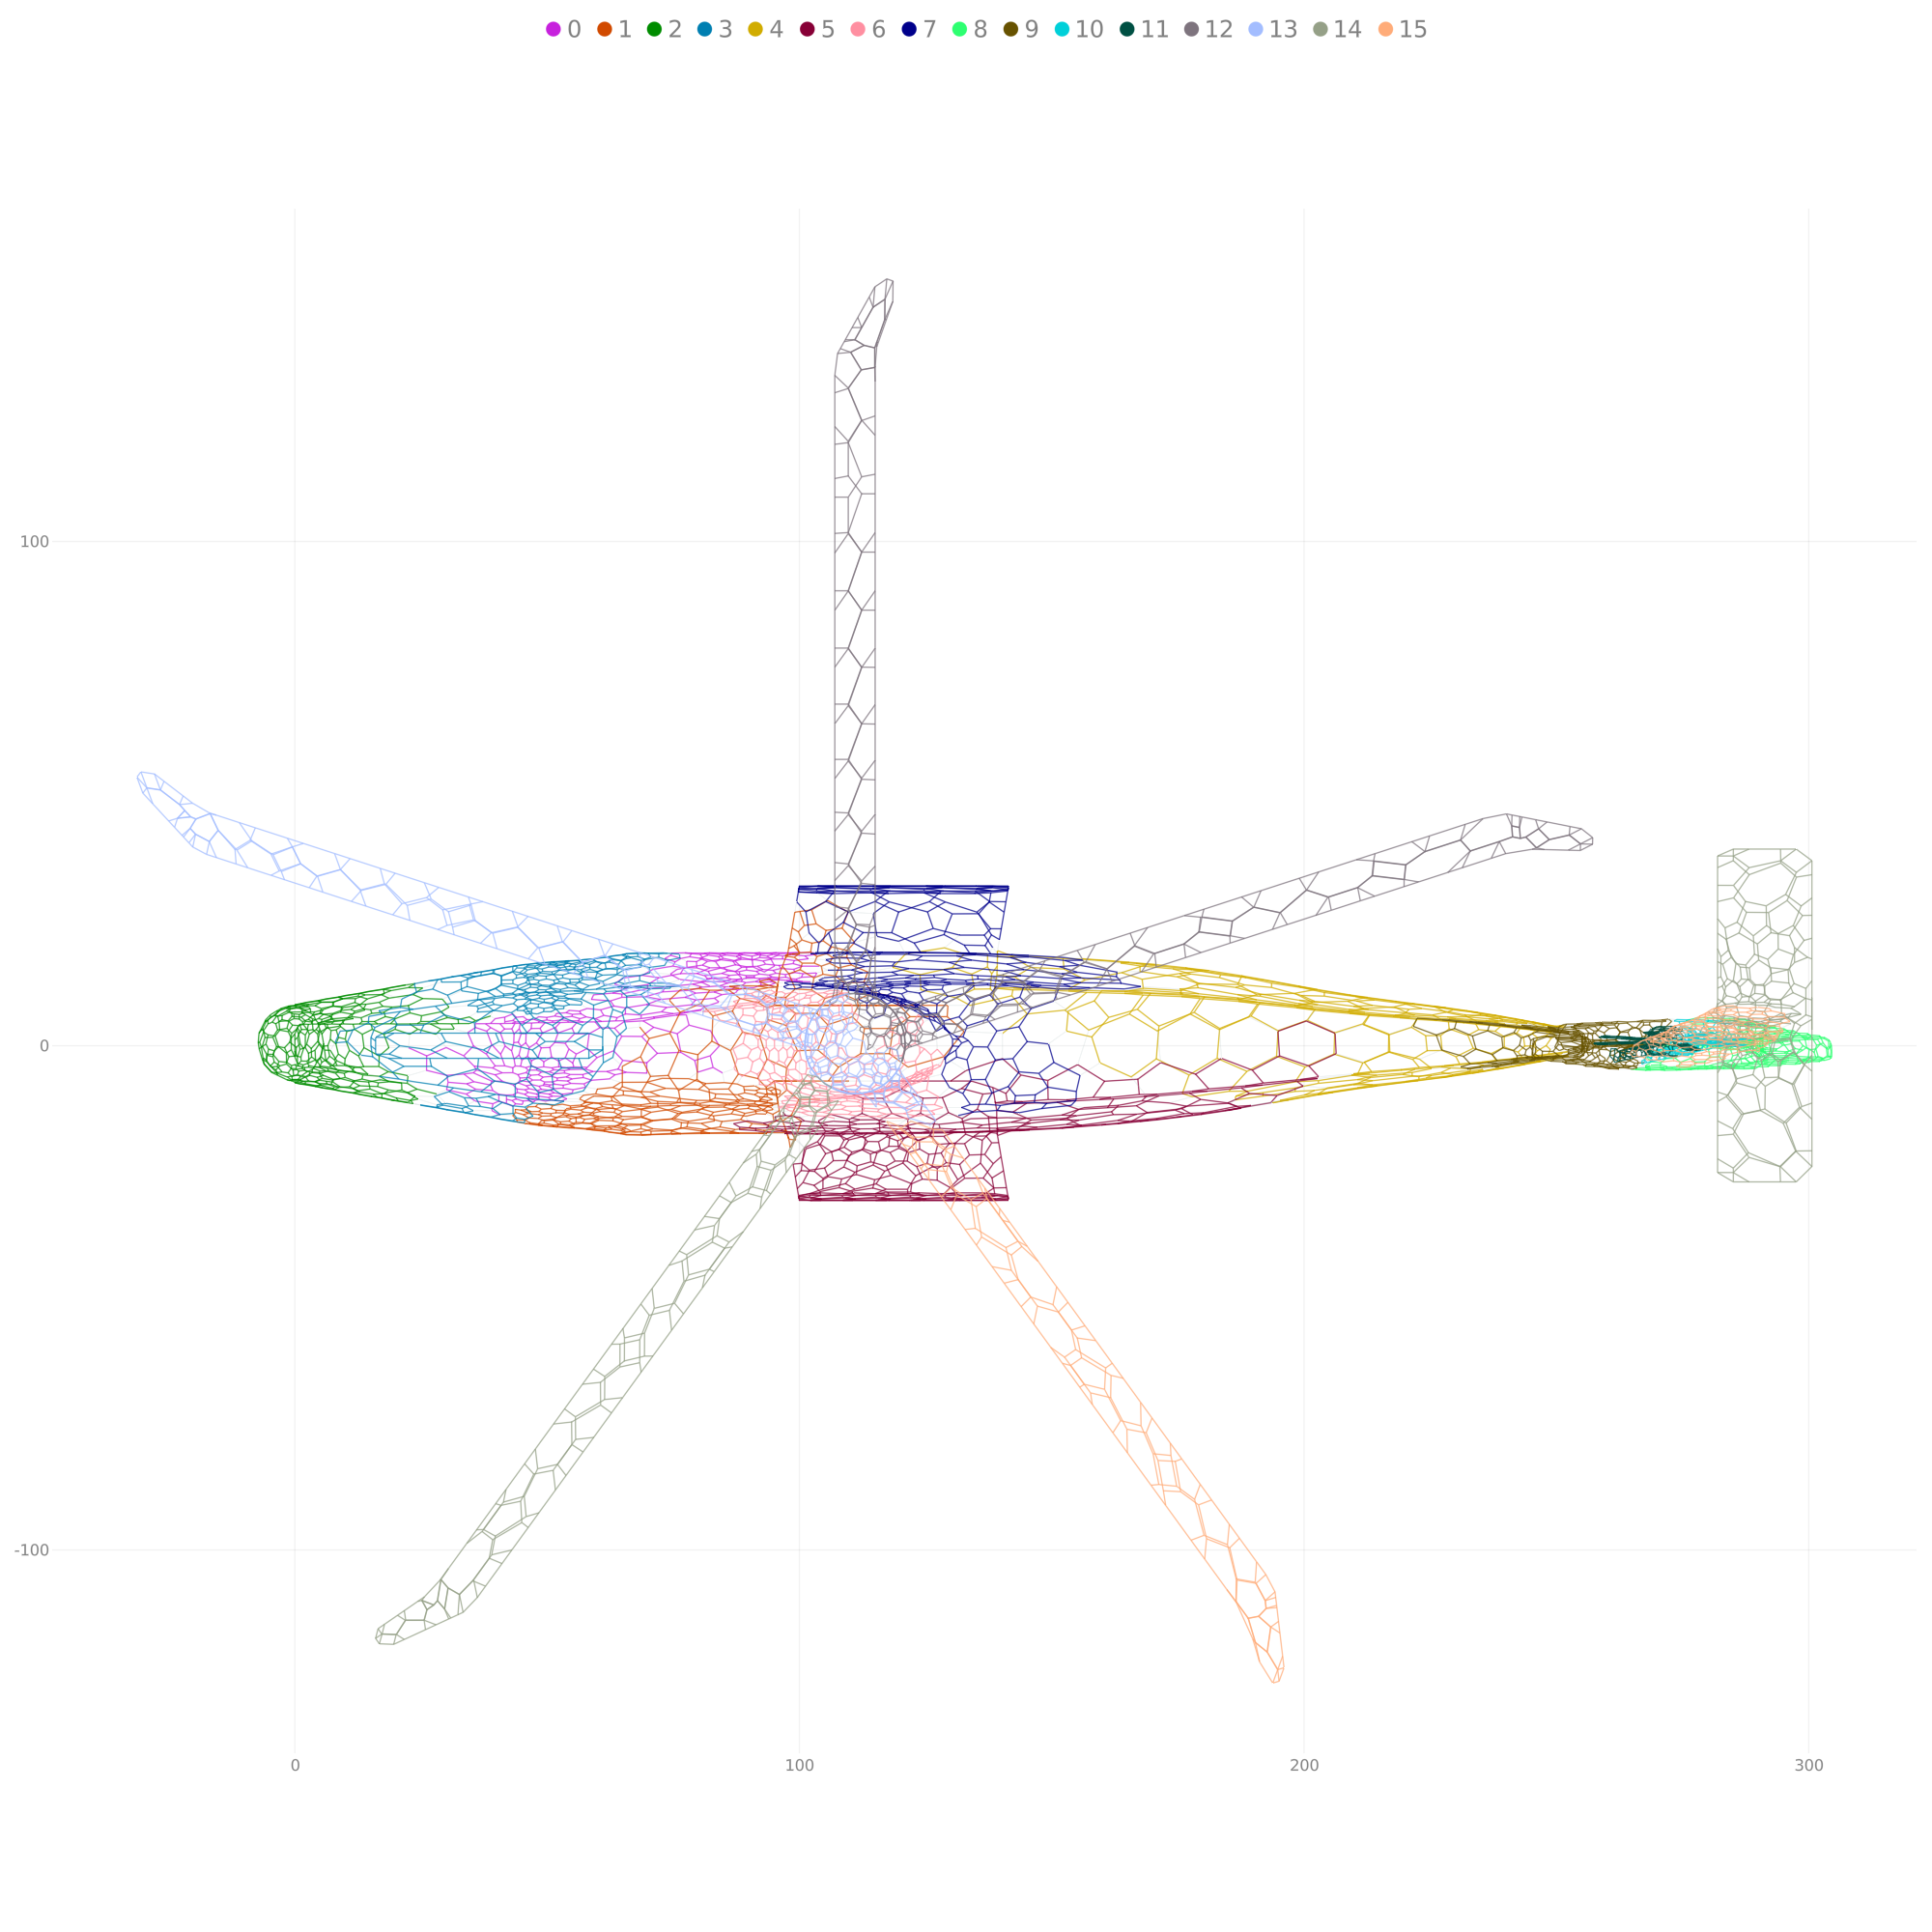
\includegraphics[height=5cm]{fig/plot/metis/metis-commanche_dual-recursive-p16-cut_377.0.png}
        \caption{Recursive partitioning.\\\textbf{377 edge cuts}}
    \end{minipage}
    \caption*{Partitioning comparison for mesh $\texttt commanche\_dual$ with $n=4$ (16 partitioned subgraphs)}
\end{figure}
\begin{figure}[h!]
    \begin{minipage}{0.5\textwidth}
        \centering
        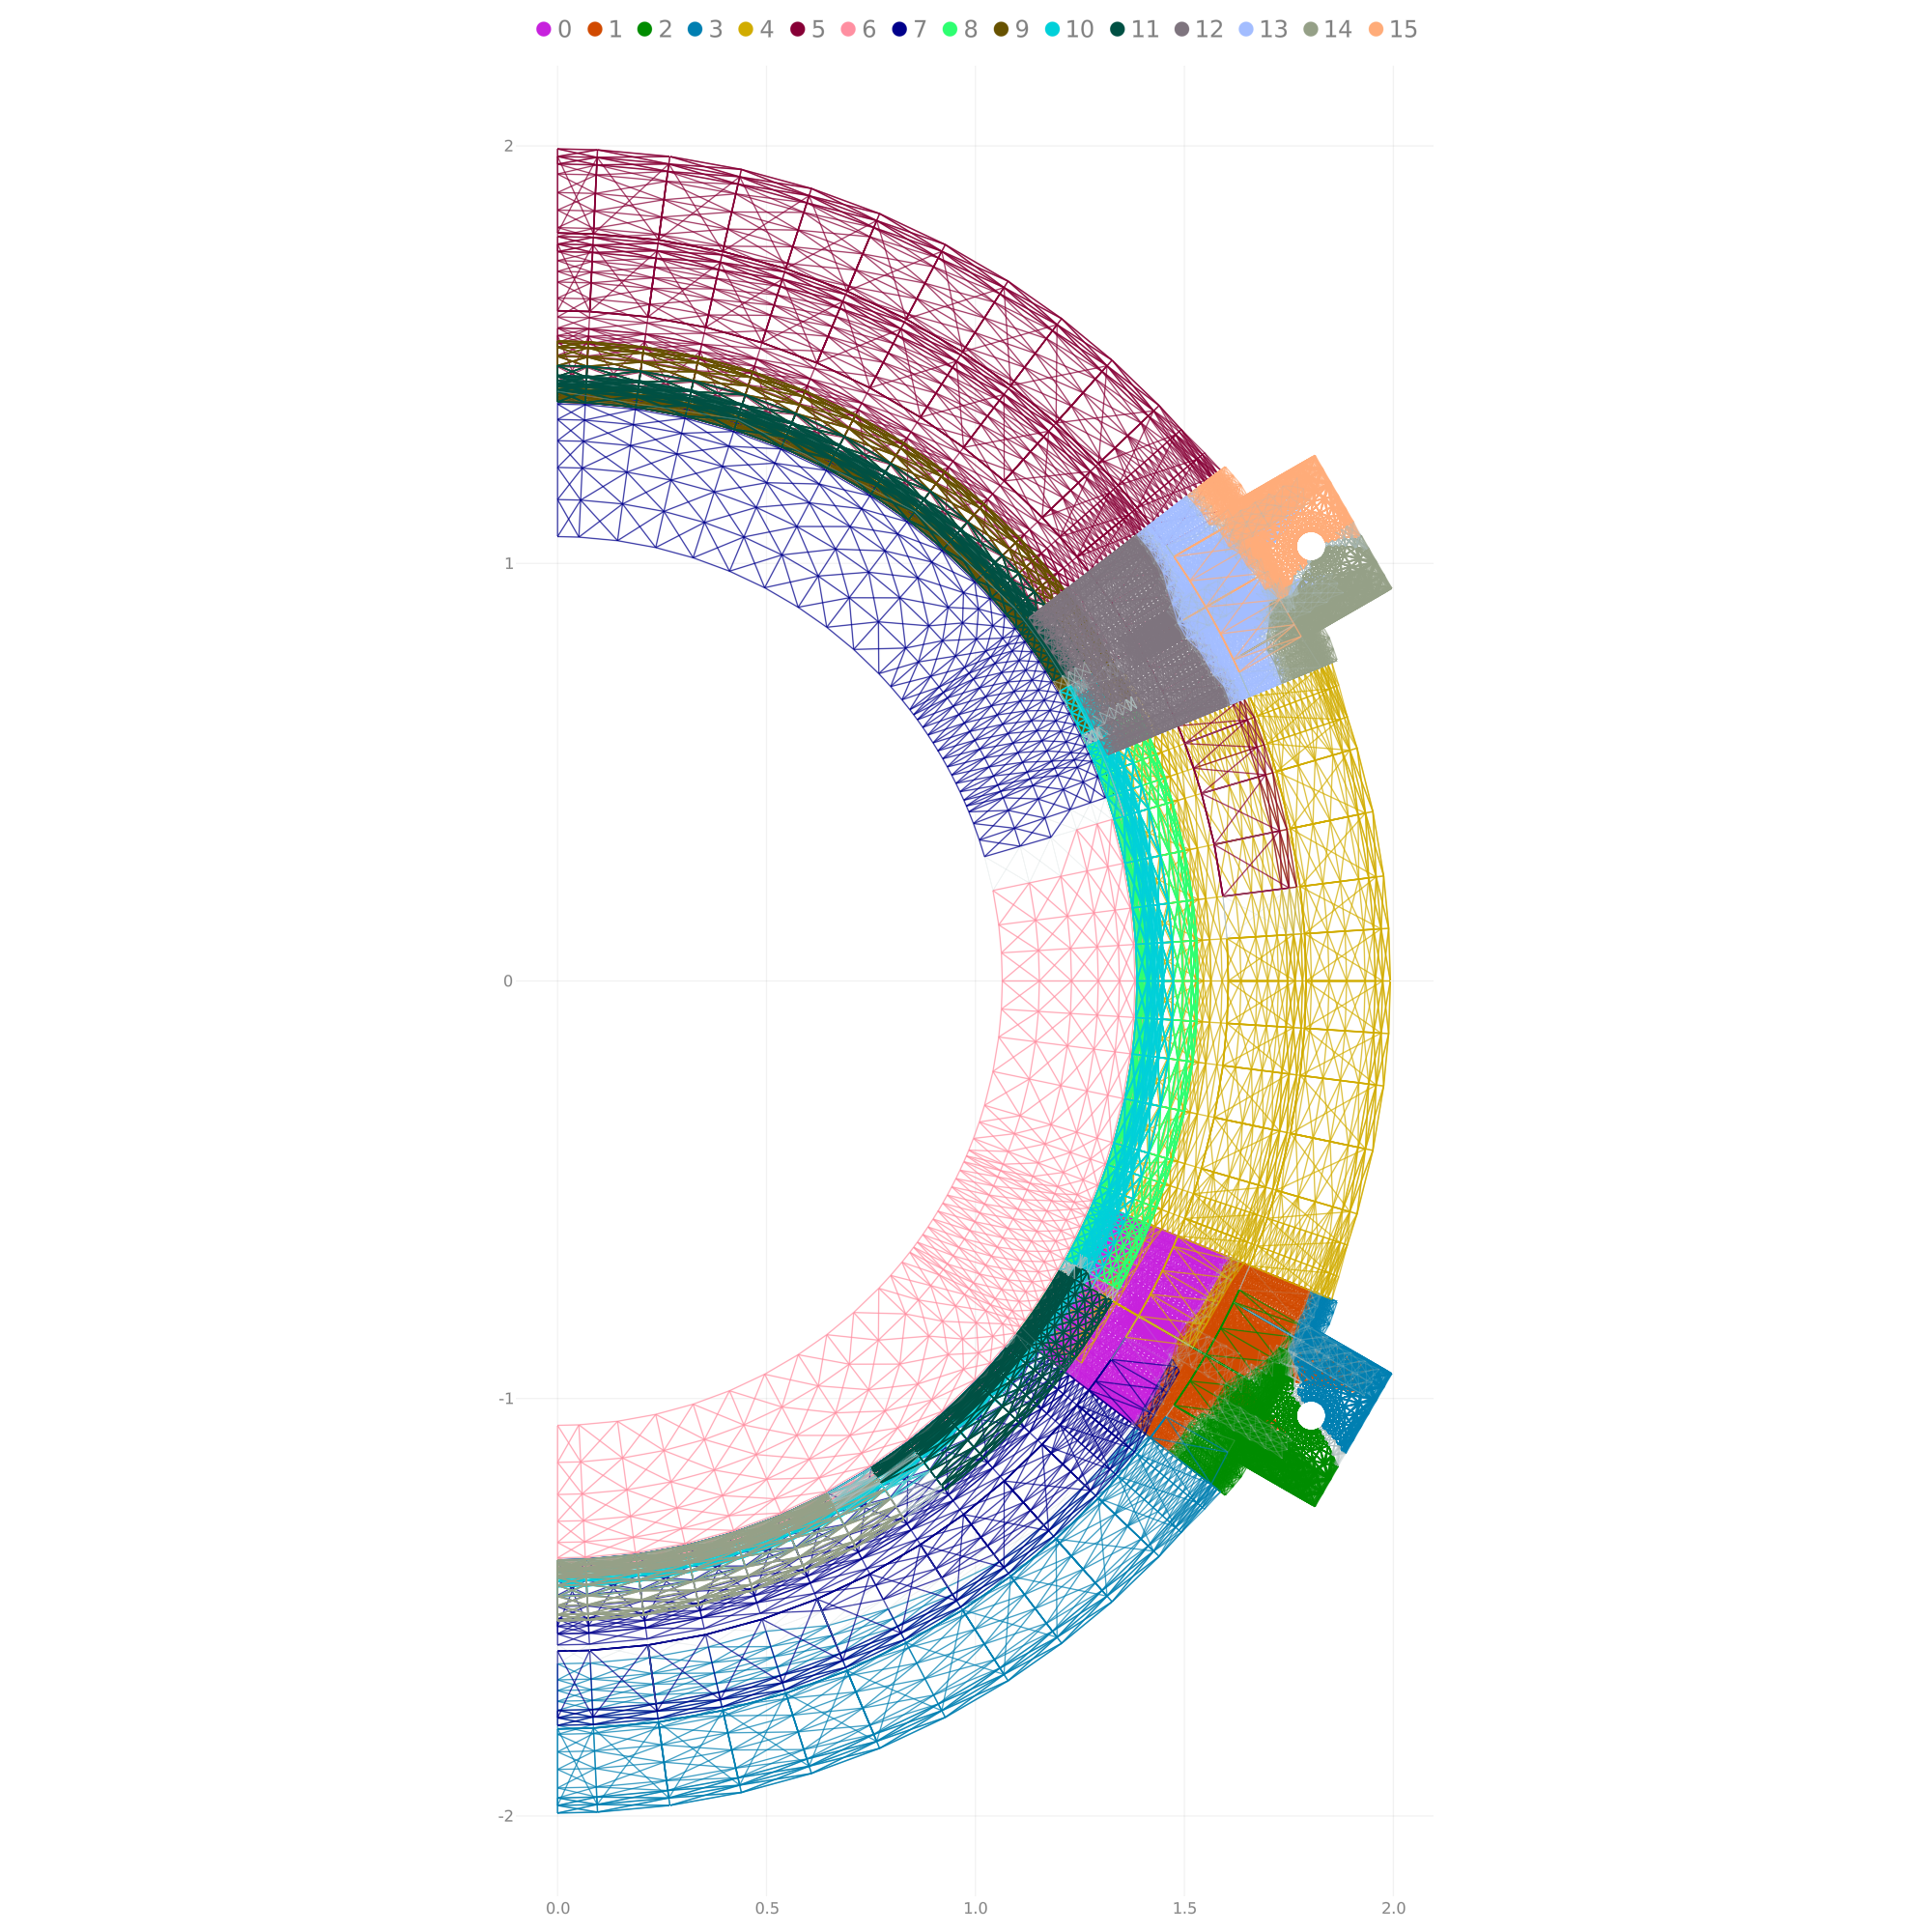
\includegraphics[height=5cm]{fig/plot/metis/metis-skirt-kway-p16-cut_3307.0.png}
        \caption{$k$-way partitioning .\\\textbf{3307 edge cuts}}
    \end{minipage}
    \begin{minipage}{0.5\textwidth}
        \centering
        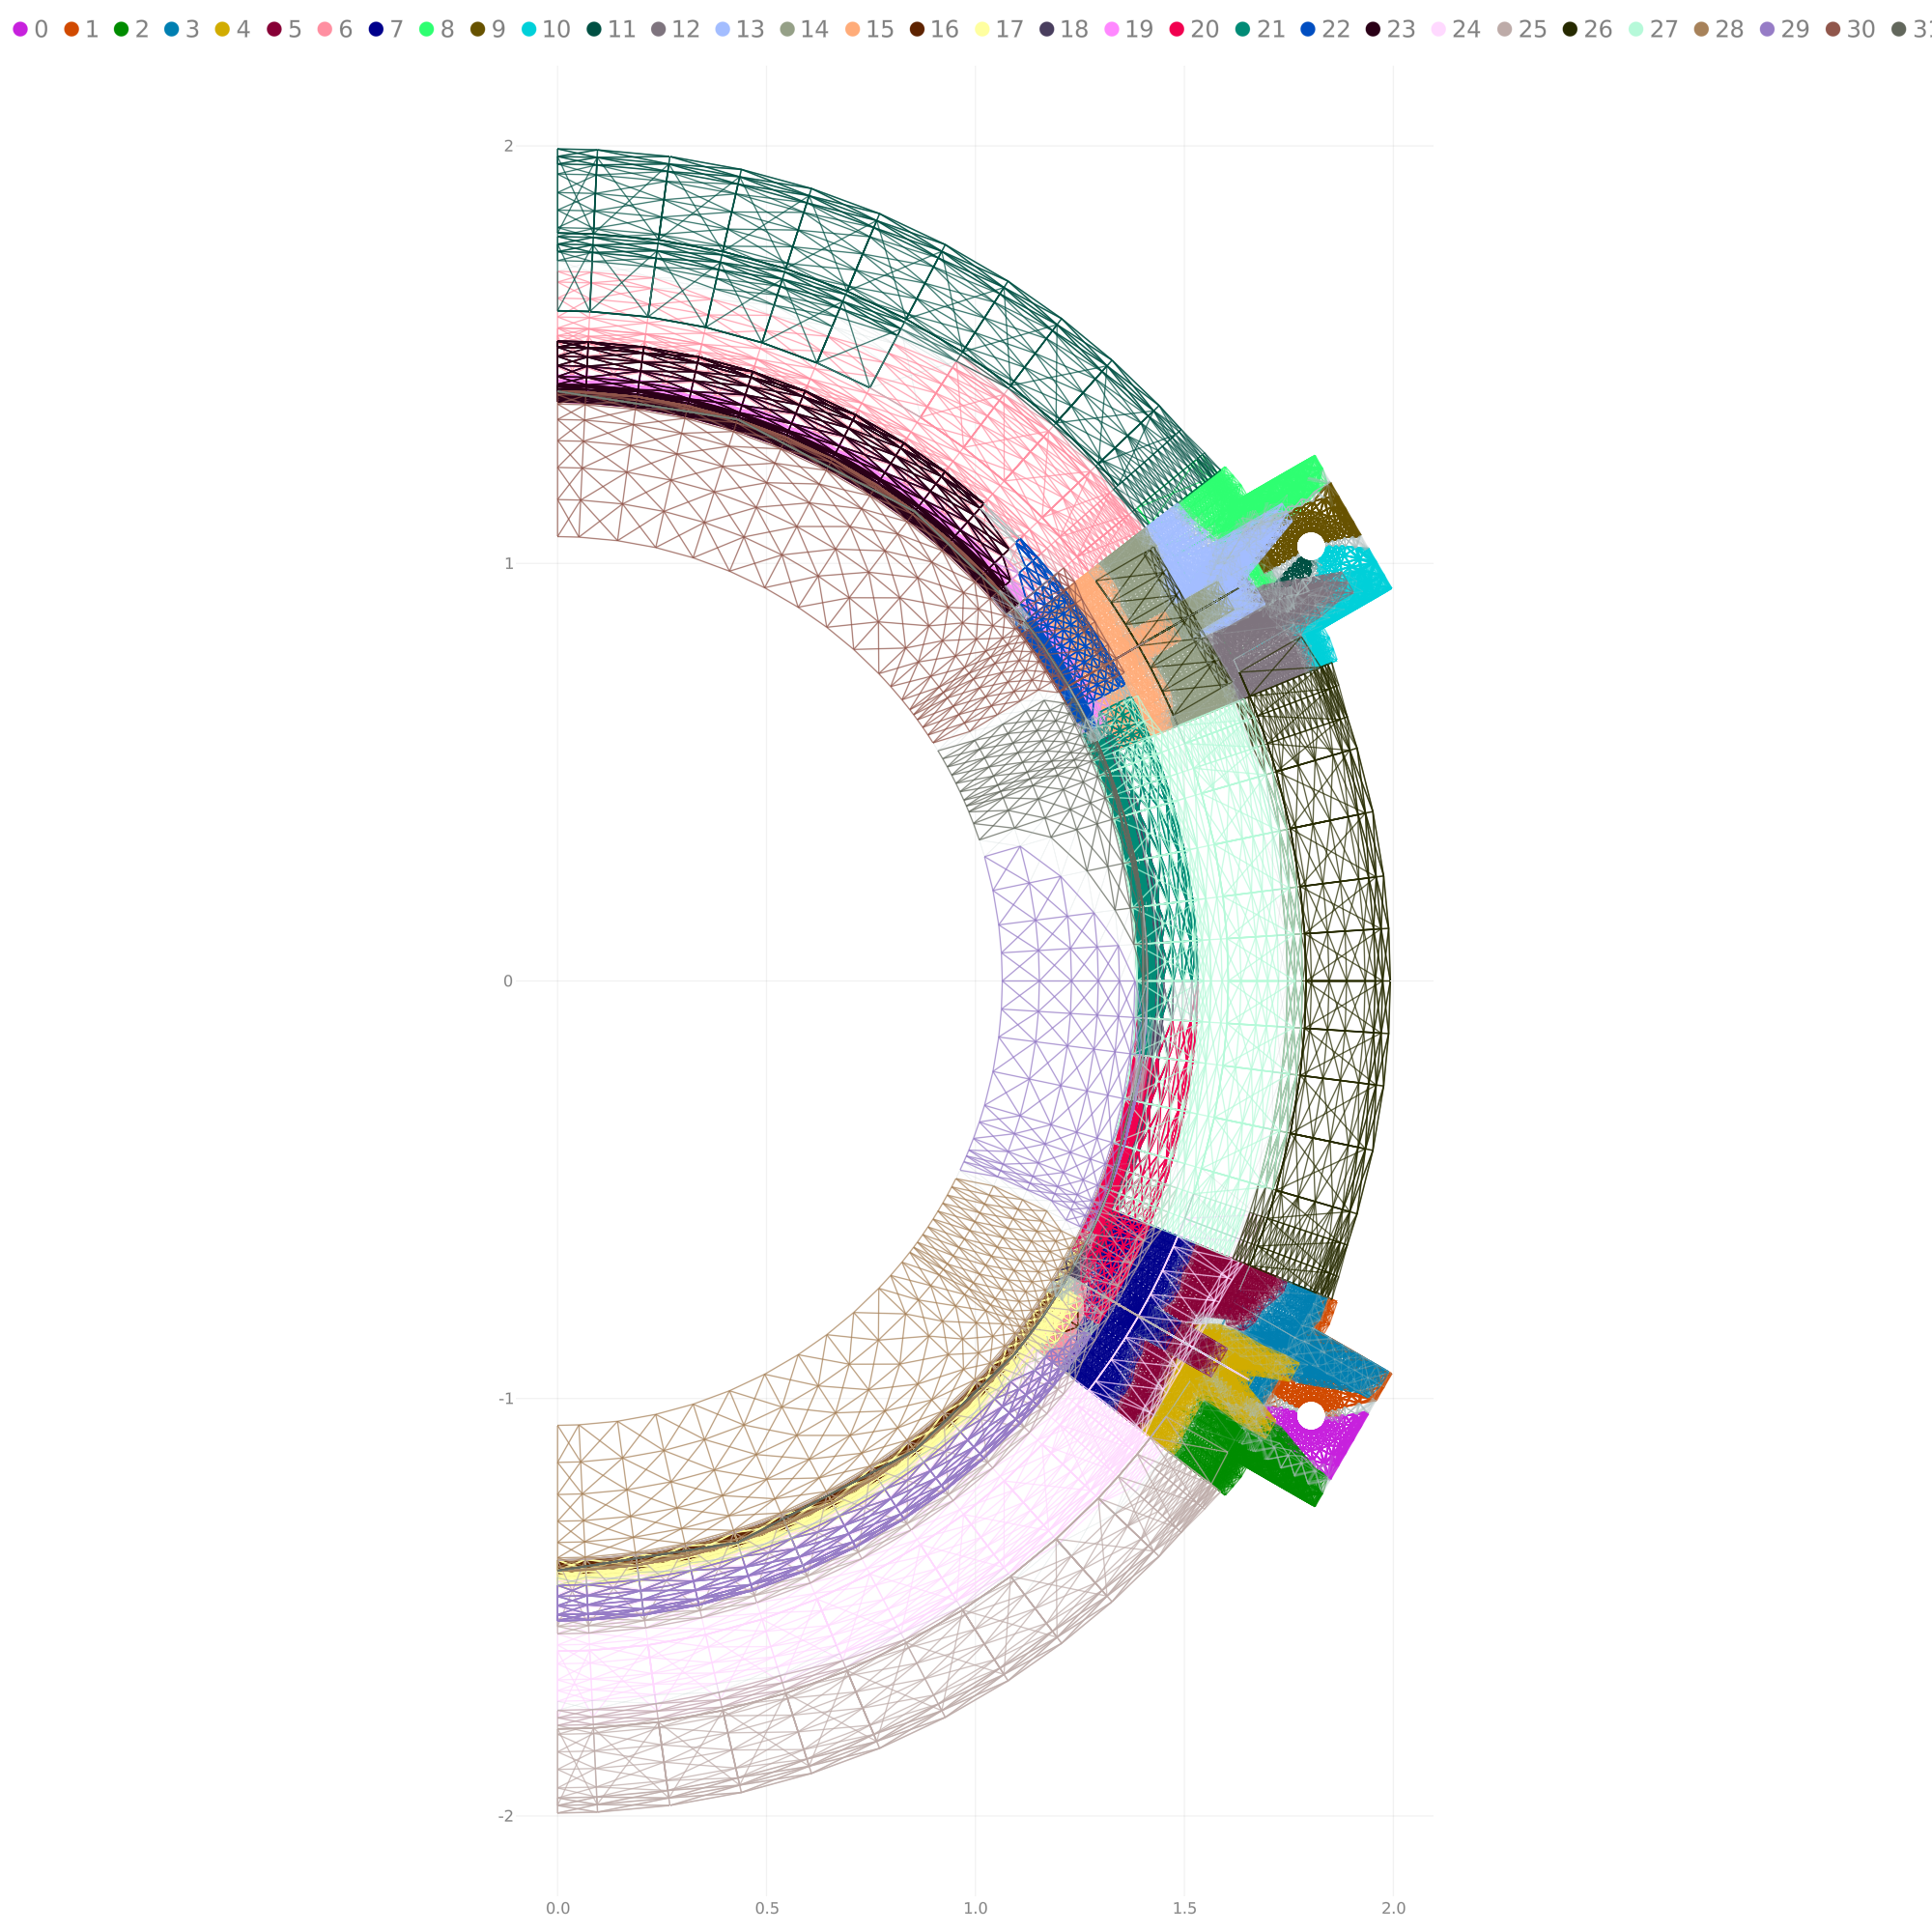
\includegraphics[height=5cm]{fig/plot/metis/metis-skirt-recursive-p16-cut_6364.0.png}
        \caption{Recursive partitioning.\\\textbf{3262 edge cuts}}
    \end{minipage}
    \caption*{Partitioning comparison for mesh $\texttt skirt$ with $n=4$ (16 partitioned subgraphs)}
\end{figure}

\begin{table}[h!]
\centering
\begin{tabular}{l|r|r} \hline\hline 
              Partitions & Helicopter &  Skirt \\
\hline
  16-recursive bisection &      377.0 & 3262.0 \\
 16-way direct bisection &      336.0 & 3307.0 \\
  32-recursive bisection &      578.0 & 6364.0 \\
 32-way direct bisection &      528.0 & 6095.0 \\
 \hline \hline
\end{tabular}              
\label{table:Compare_Metis}
\end{table}

\end{document}